\documentclass[12pt]{scrreprt}
\usepackage{fontspec,microtype}
\usepackage[ngerman]{babel}
\usepackage[utf8]{inputenc}
\usepackage[T1]{fontenc}
\usepackage{ae}
\usepackage{graphicx}
\usepackage{hyperref}
%\usepackage[printonlyused,withpage]{acronym}
\usepackage[acronym,toc,section]{glossaries}
\usepackage{subfig}
\usepackage{setspace}
\usepackage{xcolor}

\usepackage{geometry}
\geometry{a4paper, top=15mm, left=35mm, right=25mm, bottom=15mm}

%Fancy Kapitelübersxchrift und Textfont
\usepackage{lmodern,titlesec,tikz,blindtext}
\newcommand*{\chapnumfont}{\normalfont\huge\bfseries}
\titleformat{\chapter}[display]
{\filleft\bfseries}
{\filleft%
  \begin{tikzpicture}
    \draw[fill,color=black] (0,0) rectangle (2cm,2cm);
    \draw[color=white] (1cm,1cm) node {\chapnumfont\thechapter};
  \end{tikzpicture}
}
{20pt}
{\Huge}
\setmainfont{Minion Pro}
\setsansfont{Myriad Pro}

\newglossary[slg]{symbolslist}{syi}{syg}{Symbolverzeichnis}
\renewcommand*{\glspostdescription}{}
\makenoidxglossaries
%Befehle für Symbole
\newglossaryentry{symb:Pi}{
name=$\pi$,
description={Die Kreiszahl.},
sort=symbolpi, type=symbolslist
}


%Befehle für Abkürzungen
\newacronym{acr:AR}{AR}{Augmented Reality}
\newacronym{acr:VR}{VR}{Virtual Reality}
\newacronym{acr:UE}{UE}{Unity Engine}
\newacronym{acr:UE4}{UE4}{Unreal Engine 4}
\newacronym[plural={\glspl{glos:SDK}}]{acr:SDK}{SDK}{\gls{glos:SDK}}
\newacronym{acr:knn}{KNN}{Künstliche Neuronale Netze}
\newacronym{acr:UI}{UI}{User Interface}
\newacronym{acr:IDS}{IDS}{Interne Datenstruktur}


\newglossaryentry{glos:SDK}{%
  name={Software Development Kit},
  description={TODO},
  plural={Software Development Kits}
}

\newglossaryentry{glos:Workflow}{%
  name={Workflow},
  description={TODO},
}

\newglossaryentry{glos:OpenSrc}{%
  name={Open Source},
  description={TODO},
}

\newglossaryentry{glos:Labeling}{%
  name={Labeling/Datennotation/Klassifizierung},
  description={TODO},
  plural={Labeln}
}

\newglossaryentry{glos:Tiefenkamera}{%
  name={Tiefenkamera},
  description={TODO},
  plural={Tiefenkameras}
}

\newglossaryentry{glos:Umfeldmodell}{%
  name={Tiefenkamera},
  description={TODO},
  plural={Umfeldmodelle}
}

\newglossaryentry{glos:Roomscaling}{%
  name={Roomscaling},
  description={TODO}
}

\newglossaryentry{glos:Debugger}{%
  name={Debugging-Tool},
  description={TODO},
  plural={Debugging-Tools}
}

\newglossaryentry{glos:Taktrate}{%
  name={Taktrate},
  description={TODO}
}

\newglossaryentry{glos:UI}{%
  name={User Interface},
  description={TODO},
  plural={User Interfaces}
}

\newglossaryentry{glos:Scripting}{%
  name={Scripting},
  description={TODO}
}

\newglossaryentry{glos:PostPr}{%
  name={Post Processing},
  description={TODO}
}

\newglossaryentry{glos:Shader}{%
  name={Shader},
  description={TODO}
}

\newglossaryentry{glos:GameEngine}{%
  name={Game Engine},
  description={TODO}
}

\newglossaryentry{glos:PredAna}{%
  name={Predictive Analytics},
  description={TODO}
}

\makeindex


\begin{document}
\onehalfspacing
%\sffamily


\title{
	{Entwicklung einer VR-basierten Methode für 3D-Datennotation}\\
	{\large Cmore Automotive GmbH}\\
	{
\includegraphics{Main_Images/cmoreLogo}}
}
\author{Patrick Grüner}
\date{\today}
\maketitle

\pagenumbering{roman}
\tableofcontents

\newpage
\chapter*{Abstract}
Abstract goes here

\chapter*{Dedication}
To mum and dad

\chapter*{Declaration}
I declare that..

\chapter*{Acknowledgements}
I want to thank...
\newpage

\newpage
\printnoidxglossary[style=altlist,title=Glossar]

\newpage
\deftranslation[to=German]{Acronyms}{Abkürzungsverzeichnis}
\printnoidxglossary[type=\acronymtype,style=long]

\newpage
\printnoidxglossary[type=symbolslist,style=long]

\newpage

\pagenumbering{arabic}
\chapter{Einleitung}
\graphicspath{{Kapitel/Kapitel1_Einleitung/Images/}}

Der Einsatz künstlicher Intelligenzen ist aktuell in allen Bereichen der Informatik auf dem Vormarsch. Dies gilt vor allem für die Automobilindustrie, da das Thema des autonomen Fahrens nicht ohne intelligente Algorithmen realisierbar ist. Eine wichtige Rolle bei der Entwicklung solcher Algorithmen spielt dabei das maschinelle Lernen. Dabei wird versucht, ausgehend von vielen lehrreichen Beispieldaten, die Lösung einer Aufgabe zu lernen und auf andere unbekannte Daten zu verallgemeinern. So kann ein System auch auf vorher ungesehene Daten reagieren, was mit einer statischen Programmierung nur schwer oder gar nicht möglich ist. Der Erfolg dieses Prinzips hängt genauso von der Qualität der Trainingsdaten ab wie der des Algorithmus. Deshalb wird in die Erstellung dieser Daten sehr viel Arbeit gesteckt.\\

Im Bereich der Fahrerassistenzsysteme und des autonomen Fahrens ist es wichtig, dass das Auto seine Umgebung so gut wie möglich wahrnehmen kann. Deshalb werden für Algorithmen, die in diesen Bereichen angewendet werden, Daten von Sensoren verwendet um das Umfeld des Autos wahrzunehmen. Dies sind meist Kamera-, Rader- oder Lidarsensoren. Die Eingangsdaten dieser Sensoren müssen nun so aufbereiten werden, damit ein lernendes Computersystem etwas damit anfangen kann. Dazu werden alle, für das Anwendungsfeld wichtigen Teile mit entsprechenden Klassifikationen versehen. Diese Klassifikationen werden auch als \textit{Labels} oder \textit{Annotationen} bezeichnet. Zum Beispiel werden auf einem Kamerabild alle Personen und Fahrzeuge als eben diese markiert. Das Fahrzeug kann auf diese Weise lernen wie Personen und Fahrzeuge aussehen, um sie dann später im Straßenverkehr selbstständig wiederzuerkennen. Radar- und Lidarsensoren liefern stattdessen Punktwolken als Eingangsdaten (vgl. Abbildung \ref{fig:Punktwolke}), das Prinzip bleibt allerdings das gleiche. Auch hier müssen alle wichtigen Teile, in diesem Fall Punkte, mit entsprechenden Klassen versehen werden. Dieser Vorgang nennt sich \textit{Labeln} bzw. \textit{Annotieren}.\\

\begin{figure}%
	\centering
    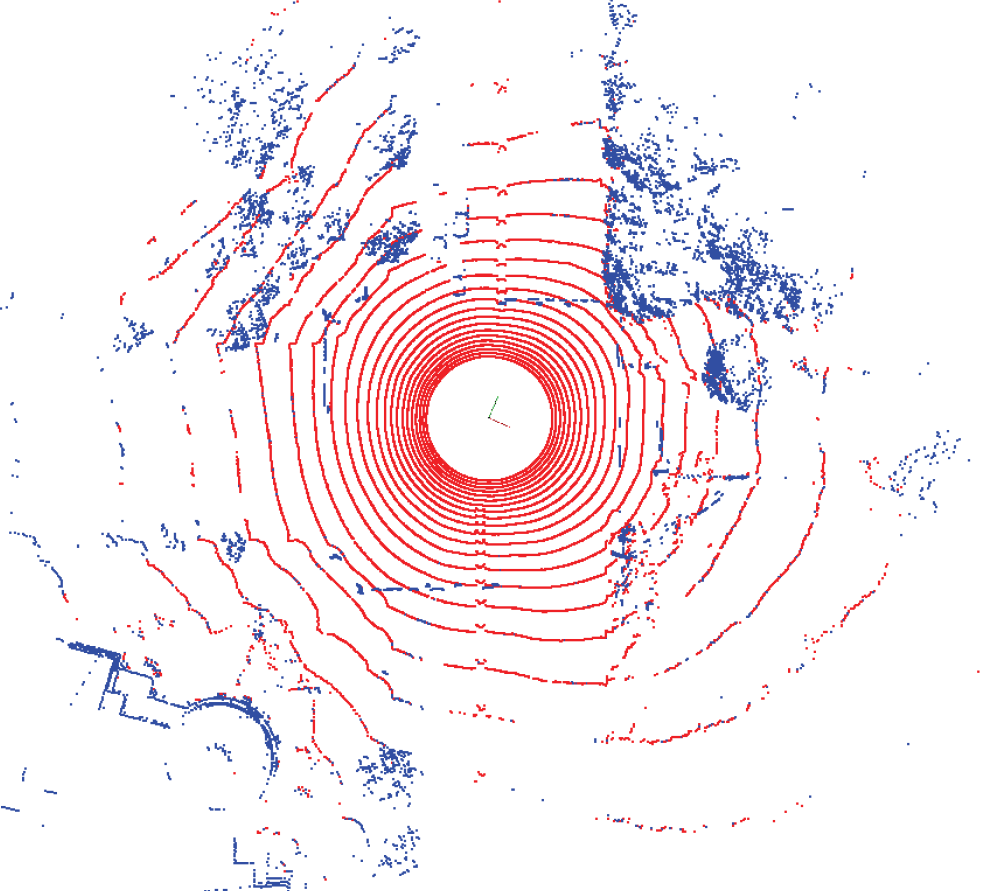
\includegraphics[width=7.5cm]{Punktwolke}
    \caption{Vogelperspektive auf eine Lidar-Punktwolke, wobei die roten Punkte alle Boden- und die blauen alle Nicht-Bodenpunkte darstellen \cite{bib:FastGroundSeg}}
	\label{fig:Punktwolke}
\end{figure}


\section{Motivation}
In einem bislang aufwändigen Verfahren (siehe Kapitel \ref{sec:C.LABEL}) müssen diese Punktwolken so aufbereitet und mit einer Bedeutung versehen werden, dass die Algorithmen an diesen Beispielen etwas lernen können. Sie müssen nach dem Lernen in der Lage sein Unterscheidungen und Erkennungen selbst durchzuführen und dabei möglichst wenige Fehler machen. Bei solchen Verfahren kommen Softwareanwendungen wie \textit{C.LABEL} zum Einsatz. Dies ist eine Anwendung zum Annotieren verschiedener Sensordaten für den Automobilbereich und wurde von der Firma \textit{CMORE Automotive GmbH} entwickelt. CMORE ist das betreuende Unternehmen dieser Masterarbeit und wird in Kapitel \ref{sec:CMORE} vorgestellt. Das Programm C.LABEL ist in Kapitel \ref{sec:C.LABEL} erklärt. C.LABEL ist eine Anwendung, die zunächst die Sensordaten für den menschlichen Benutzer visualisiert. Dieser muss sie dann manuell mit unterschiedlichen Bedeutungen versehen. Wegen der großen Menge an Daten, die für das Trainieren der Algorithmen benötigt wird, muss dieses manuelle Annotieren möglichst effizient durchführbar sein.\\

Ein zweidimensionales Kamerabild kann sehr einfach auf einem Computermonitor dargestellt und bearbeitet werden. Eine besondere Herausforderung stellt jedoch die Verarbeitung von 3D-Daten, wie einer Punktwolke, dar. Hier stößt man mit den Möglichkeiten eines zweidimensionalen Computermonitors schnell an die Grenzen einer effizienten Darstellung und Bearbeitung. So ist es beispielsweise für die Annotierung solcher Punktwolken und ihrer Einzelmesswerte schwierig, die optimale Perspektive auf die Daten zu finden, die eine effiziente Erfassung durch den Menschen und eine entsprechende Bearbeitung zulässt. Dies erfordert von den Benutzern sehr viel Übung und Erfahrung, durch entsprechende Drehungen der Punktwolkendarstellung sich in dieser zurechtzufinden und Messpunkte realen Objekten zuzuordnen.\\ 

Eine Alternative dazu soll diese Masterarbeit bieten, welche eine Applikation beschreibt, die das Visualisieren und Annotieren von Punktwolken einfacher und effizienter gestaltet. Mittels neuartiger Technologien wie Virtual- und Augmented Reality soll die Grenze zwischen 2-D und 3-D aufgehoben werden, sodass man sich als interaktiver Teilnehmer im dreidimensionalen Raum durch die Sensordaten navigieren, mit ihnen interagieren und sie annotieren kann.\\

\section{Ziel der Arbeit}
Ziel dieser Arbeit ist es zunächst ein passendes Medium für eine solche Applikation zu finden, das nicht nur die Anforderungen der Applikation selbst erfüllt, sondern auch an einem handelsüblichen Büro-Arbeitsplatz verwendet werden kann. Anschließend soll eine Applikation erstellt werden die folgende Grundfunktionalität erfüllt:\\

\begin{enumerate}
\item Mit der Anwendung soll es Möglich sein ein, bei CMORE gängiges, Datenformat einzulesen und alle nötigen Informationen daraus zu extrahieren

\item Aus den extrahierten Informationen soll eine Punktwolke generiert und innerhalb des gewählten Mediums visualisiert werden.

\item Der Benutzer muss die Möglichkeit haben durch die Punktwolke zu navigieren.

\item Die Applikation muss die Möglichkeit bieten jeden einzelnen Punkt mit einer Klassifikation versehen zu können. Dabei sollen Alleinstellungsmerkmale des gewählten Mediums benutzt werden, um eine vorzeigbare Verbesserung gegenüber der herkömmlichen Computer-Monitor-Annotation zu generieren. 

\item Alle getätigten Annotationen müssen in die eingelesenen Dateien zurückgeschrieben bzw. in neue Dateien exportiert werden.
\end{enumerate}

Anschließend sollen die Basisfunktionen erweitert und zusätzliche Funktionen hinzugefügt werden. Abhängig von der verbleibenden Zeit soll die Anwendung gemäß folgender Priorität erweitert werden:\\

\begin{enumerate}
\item Es sollen neue Möglichkeiten zur Annotation von Punkten implementiert werden.

\item Die Möglichkeit, eigene Klassifikationen für Punkte zu erstellen, soll hinzugefügt werden.

\item Neue Datenformate importieren.

\item Neue Navigationsmöglichkeiten implementieren.
\end{enumerate}

Am wichtigsten wäre hierbei also die Applikation um effiziente Möglichkeiten zum labeln von Punkten zu erweitern. Außerdem sollte es für den Benutzer möglich sein individuelle Klassifikationen anzulegen, um unterschiedliche Anwendungsgebiete abzudecken. Optional sind neue Navigationsmöglichkeiten und einlesbare Datenformate. 

\section{Umfeld der Arbeit}

\subsection{CMORE Automotive GmbH}
\label{sec:CMORE}

\subsection{C.LABEL}
\label{sec:C.LABEL}


\chapter{Vorbereitungen}
\graphicspath{{Kapitel/Kapitel2_Vorbereitungen/Images/}}

%TODO
Kurze Einleitung was alles vorbereitet wurde.

\section{Wahl des passenden Mediums} 
Um das \glslink{glos:Labeling}{Labeling} von Daten, insbesondere Punktwolken, im dreidimensionalem Raum zu verwirklichen, gibt es zwei wesentliche Technologien die dafür relevant erscheinen. Diese sind \acrfull{acr:AR} und \acrfull{acr:VR}.\\

Unter \acrlong{acr:AR} versteht man die direkte oder indirekte Sicht auf die reale, physische Welt, welche durch digitale Inhalte erweitert wird. Dies wird vor allem durch Smartphones oder \acrshort{acr:AR}-Brillen realisiert. Bei einem Smartphone hat man beispielsweise einen indirekten Blick auf die reelle Umgebung durch das Display, welches ein Live-Bild der Kamera anzeigt. Diesem Bild können nun digitale Inhalte hinzugefügt werden. Bei einer Brille (vgl. Abbildung \ref{fig:AR-Brillen}) sieht man durch die Gläser direkt auf die physische Welt. Hierbei fungieren die Gläser als Display, welche in der Lage sind holographische Objekte anzuzeigen. Dies führt zu einer, für den Benutzer, sehr immersiven Vermischung der realen und der digitalen Welt. Üblicherweise ist es bei diesen Brillen sogar möglich durch Gesten, die mittels Händen durchgeführt werden, mit den Hologrammen zu interagieren.\\

\acrlong{acr:VR} ist eine Technologie bei der spezielle \acrshort{acr:VR}-Brillen zum Einsatz kommen, welche keine Sicht mehr auf die reale Umgebung ermöglichen (vgl. Abbildung \ref{fig:VR-Brillen}). Das Blickfeld des Menschen wird hierbei komplett von einem Display abgedeckt, das sich im Inneren der Brille befindet. So kann dem Benutzer eine komplette virtuelle Welt angezeigt werden. Mittels kompatiblen Controllern (vgl. Abbildung \ref{fig:Oculus}) kann sich durch diese Welt bewegt bzw. mit ihr interagiert werden. Die Controller werden dabei von einem Sensor erfasst und somit können reale Bewegungen der Controller in die virtuelle Welt der Brille übersetzt werden.


\subsection{Eignung von \acrlong{acr:AR} und \acrlong{acr:VR} im Bezug auf 3D-Datennotation}
Im folgenden Abschnitt wird auf die positiven und negativen Aspekte der beiden Technologien eingegangen, um abzuwägen welche besser für \glslink{glos:Labeling}{3D-Labeling} geeignet ist.

\subsubsection{Eignung von \acrlong{acr:AR}}
Der, im Rahmen dieser Arbeit, entwickelte Prototyp zur \glslink{glos:Labeling}{3D-Datennotation} ist nicht nur als Nutzungssoftware geplant, sondern dient auch als Anschauungsmaterial, beispielsweise für Messen. Zieht man diese Tatsache in Betracht, eignet sich \acrlong{acr:AR} sehr gut für diesen Zweck. Es wirkt durch die Vermischung von realen und digitalen Inhalten nämlich sehr futuristisch. Zudem ist das direkte einblenden holographischer Inhalte, durch eine \acrshort{acr:AR}-Brille, zum Zeitpunkt der Erstellung dieser Arbeit, noch wenig verbreitet (Microsoft Hololens wurde nur wenige Tausend mal verkauft \cite{bib:HololensVerkaufszahlen}), was bei unwissenden Benutzern zu einem beeindruckenden Effekt führt. Des Weiteren bietet die \acrlong{acr:AR} Technologie viele, für zukünftige \glslink{glos:Labeling}{Labeling}-Methoden relevante, Möglichkeiten. Den heutigen \acrshort{acr:AR}-Brillen ist es durch \glspl{glos:Tiefenkamera} möglich Objekte und deren Distanzen zur Brille wahrzunehmen. Folglich könnte ein zukünftiger Ansatz sein, eine Punktwolke der Umgebung, wie sie in \ref{sec:C.LABEL} zu sehen ist, mit einer \acrshort{acr:AR}-Brille zu erstellen. Diese kann anschließend vor Ort, in der Umgebung in der die Punktwolke erstellt wurde, klassifiziert werden.\\ %TODO Dieser Ansatz könnte ausführlicher sein. 

Ein wichtiger Punkt der ebenfalls betrachtet werden muss ist die Bedienung der Brille bzw. die Interaktion mit den digital dargestellten Objekten und Informationen. Die Steuerung von \acrshort{acr:AR}-Brillen erfolgt handelsüblich über Gesten, welche mit der Hand bzw. den Händen getätigt werden. Ob diese Art der Interaktion für den hier gewünschten Anwendungsfall passend wäre, lässt sich im Voraus schwer feststellen. Denkbar wäre, dass sich der Benutzer durch intuitive Gesten, die man auch bei realen Objekten nutzt, schnell an die Bedienung des Tools gewöhnen würde. Andererseits könnte die Selektion der Elemente einer Punktwolke zu ungenau sein, da die Brille die Position der Hand nicht richtig interpretiert bzw. diese nicht richtig zur Position der digitalen Inhalte interpretiert. Eine genaue Einschätzung der Bedienung für solch einen Anwendungsfall kann allerdings nur gegeben werden indem man einen \glslink{glos:Labeling}{Labeling}-Prototypen erstellt und ihn anschließend über längere Zeit testet. Dies ist im Zeitrahmen einer Masterarbeit jedoch nicht möglich. Falls sich nämlich die Steuerung als ungeeignet herausstellt bleibt nicht genug Zeit für eine Neuentwicklung auf einer anderen Plattform.\\  

Darüber hinaus gibt es natürlich auch Aspekte die gegen die \acrshort{acr:AR}-Technologie sprechen. Die \glslink{glos:Labeling}{Klassifizierung} einer Punktwolke mit dieser Technik ist an einem normalen Büro-Arbeitsplatz nicht möglich, zumindest nicht in einem Maßstab in dem es sinnvoll wäre. Die holographischen Punkte kollidieren, wenn sie darauf programmiert sind, mit der Umgebung und so würde Darstellung des \glslink{glos:Umfeldmodell}{Umfeldmodells} verfälscht werden. Auch wenn sie das nicht tun, dann wäre die Umgebung selbst immer noch ein Hindernis für den Benutzer, denn man möchte sich ja durch die Punktwolke bewegen. Des Weiteren sind bei \acrshort{acr:AR}-Brillen die vorherrschenden Lichtbedingungen ein großer Faktor, welche die Funktionalität gewisser Anwendungsfälle beeinflussen können. Wird beispielsweise eine Lichtquelle zu sehr von einem Objekt reflektiert, kann dieses von der \gls{glos:Tiefenkamera} der Brille nicht mehr richtig erfasst werden. Somit stimmt das \gls{glos:Umfeldmodell} nicht mehr mit der Realität überein. Zudem wird nicht nur die Funktionalität von Lichteinflüssen gestört, sondern auch die Darstellung der Hologramme. Bei zu viel Licht sind diese deutlich schwerer zu erkennen, vergleichbar mit der Nutzung eines Laptops im Freien, bei dem der Bildschirminhalt wegen zu heller Umgebung ebenfalls schlecht erkennbar ist. Für die Entwicklung selbst ist es ebenfalls hinderlich das es, zum Zeitpunkt der Erstellung dieser Arbeit, wenig Dokumentationen und Hilfestellungen, zum Beispiel in Entwicklerforen, gibt. Dies ist jedoch üblich für Technologien, die noch nicht lange auf dem Markt sind. Zu guter Letzt ist noch der finanzielle Faktor zu berücksichtigen. Durch die Aktualität der Technologie ist diese auch sehr teuer. Der Preis für eine \acrshort{acr:AR}-Brille kann dabei den Betrag von 5.000 Euro überschreiten, wie im  Abschnitt \ref{sec:ARVergleich} näher erläutert wird.    

\subsubsection{Eignung von \acrlong{acr:VR}} 

Die \acrlong{acr:VR} Technologie bietet den großen Vorteil, beliebig große Räume virtuell begehbar zu machen, ohne sich in der realen Welt selbst bewegen zu müssen. Dies ermöglicht die Bewegung durch Punktwolken, die im dreidimensionalen Raum dargestellt sind, an jedem üblichen Arbeitsplatz eines Büros. Des weiteren wirkt die Steuerung der \acrshort{acr:VR}-Brillen mittels den zugehörigen Controllern zum teil sehr ausgereift. Die Positions- und Bewegungserkennung des Benutzers wird als \textit{\glqq äußerst präzise\grqq} beschrieben \cite{bib:ControllerTest}. Dies ist sehr wichtig um die Handhabung der Anwendung für den späteren Endnutzer so angenehm wie möglich zu machen. Für die Entwicklung von \acrshort{acr:VR}-Applikationen selbst ist zu sagen, dass es mittlerweile sehr Umfassende Dokumentationen, Anleitungen und Beiträge zu den jeweiligen Plattformen und \glspl{acr:SDK} gibt. Dies hängt damit zusammen, dass sich die \acrlong{acr:VR} Technologie schon etwas länger auf dem Markt befindet und die Zahl der Entwickler für \acrshort{acr:VR}-Applikationen stetig steigt. Dies ist vermutlich nicht zuletzt der Tatsache zu verdanken, dass die Preise für \acrshort{acr:VR}-Brillen gesunken sind. Wie im späteren, ausführlicher beschreibenden, Abschnitt \ref{sec:ARVergleich} gezeigt, beträgt der aktuelle Preis einer Oculus Rift 449 Euro. Sowohl die zahlreichen Informationen für Entwickler als auch der niedrige Preis der Hardware sprechen, neben den zuvor genannten Aspekten, für die Wahl von \acrlong{acr:VR} als Plattform für die Entwicklung von 3D-\glslink{glos:Labeling}{Labeling}.\\

Was mit der \acrshort{acr:VR}-Technologie nicht ohne Weiteres funktioniert, ist die physische Begehung einer, zu \glslink{glos:Labeling}{klassifizierenden}, Punktwolke. Zwar bietet die Technik die Möglichkeit durch zusätzliche Sensoren die Bewegungen des Benutzers in die virtuelle Welt zu übersetzen, jedoch funktioniert dies nur auf begrenztem Raum und ist unmöglich an einem üblichen Büro-Arbeitsplatz durchführbar. Der reale begehbare Raum muss nämlich durch diese Sensoren abgesteckt werden und ist somit durch deren Reichweite und Genauigkeit begrenzt. Ein weiter Negativaspekt ist, dass viele Benutzer von \acrshort{acr:VR}-Brillen über Übelkeit klagen. In manchen Tests sind es mehr als 50 Prozent aller Teilnehmer, vor allem wenn es sich um Frauen handelt \cite{bib:VRSickness}. 


\subsection{\acrshort{acr:AR}-Brillen im Vergleich}
\label{sec:ARVergleich}
Zum Zeitpunkt der Recherche über eine passende \acrshort{acr:AR}-Brille, gibt es zwei potentielle Geräte die in Frage kommen. Diese sind Microsofts Hololens und die Meta 2. Andere Brillen werden, aufgrund der im voraus erkennbaren Hindernisse, nicht berücksichtigt, wie beispielsweise die Google Glass, die ein viel zu kleines Display hat. Wiederum andere sind zu diesem Zeitpunkt noch nicht auf dem Markt wie das Project Aurora, welches ebenfalls von Google ist, oder die Brille castAR. Im Folgenden werden die zwei potentiellen Brillen, im Hinblick auf die Nutzung für \glslink{glos:Labeling}{3D-Datennotation}, näher analysiert.

\subsubsection{Microsoft Hololens}
Die Hololens-Brille von Microsoft (vgl. Abbildung \ref{fig:Hololens}) punktet vorwiegend in Sachen Darstellung und räumlicher Interaktion, was aus eigener Erfahrung bekannt ist. Eingeblendete Hologramme wirken auf dieser Brille sehr stabil. Ein Ruckeln oder Nachpositionieren der digital dargestellten Inhalte wurde nie bemerkt. Ebenfalls gut funktioniert die Vermessung des Raums durch die Kameras der Brille. Hologramme interagieren dadurch sehr gut mit der physischen Umgebung, indem sie beispielsweise wie ein realer Gegenstand auf dem Tisch positioniert oder an die Wand gehängt werden können. Lediglich schlecht ausgeleuchtete Bereiche eines Raumes machen dieser Funktion Probleme, sodass die Brille beispielsweise eine Wand entdeckt wo gar keine ist. Die eben genannten Merkmale der Hololens, also eine stabile Darstellung und eine gute Einbettung einer Punktwolke in einen vorhandenen Raum, ist sehr wichtig um diese zuverlässig klassifizieren zu können und somit eine gute Methode für \glslink{glos:Labeling}{3D-Datennotation} zu entwickeln.\\
%evtl eigene Erfahrung noch reinbringen

Die Gestensteuerung der Hololens wäre für den Prozess der \glslink{glos:Labeling}{Klassifizierung} von dreidimensionalen Punktwolken eher ungeeignet. Durch Kopfbewegung müsste zum gewünschte Ziel navigiert und dieses dann mit einer Tipp-Geste in der Luft ausgewählt werden. Da dieser Vorgang schon beim Eingeben eines etwas komplexeren Passwortes Probleme bereitet, wäre er bei der Klassifikation von hunderten Punkten für den Benutzer sehr mühsam und langwierig. Ein weiter Punkt der negativ ins Gewicht fällt ist das kleine Sichtfeld der Brille. Tests sprechen hierbei von einer horizontalen Sichtweite die lediglich 30 bis 40 Grad beträgt \cite{bib:HololensTest}. Der Mensch kann dagegen horizontal fast 180 Grad wahrnehmen. Diese Eigenschaft würde den Benutzer daran hindern eine Punktwolke bzw. wenigstens einen Teilbereich dieser, als ganzes wahrzunehmen. Dadurch würde ein Großteil des Reizes verloren gehen, den die \glslink{glos:Labeling}{3D-Datennotation} bietet. Zudem ist die Hololens sehr teuer. Der Preis für die  Development Edition beträgt 3.299 Euro und in der Commercial Suite-Variante kostet die Brille sogar 5.489 Euro \cite{bib:HololensPreis}. Für eine prototypische Entwicklung die im Rahmen einer Abschlussarbeit angefertigt wird, ist das für ein Unternehmen ein sehr hoher Preis.

\subsubsection{Meta 2}
Für die Meta 2-Brille (vgl. Abbildung \ref{fig:Meta2}) spricht das hohe Sichtfeld, welches dem Hersteller nach 90 Grad beträgt und laut eines Tests \textit{\glqq hält, was es verspricht\grqq} \cite{bib:Meta2Test}. Wie im vorherigen Abschnitt angemerkt, ist ein hohes Sichtfeld sehr wichtig um dem Benutzer eine immersive Sicht auf eine Punktwolke zu geben. Die Steuerung der Brille wirkt ebenfalls gut und intuitiv. So ist es möglich Hologramme durch einfaches Greifen mit einer Hand auszuwählen, ohne diese zwangsläufig mit Kopfbewegungen anzuvisieren. Dies würde das selektieren vieler holographischer Gegenstände nacheinander erleichtern. Der Preis der Meta 2 ist, im Gegensatz zur Hololens geringer. Jedoch ist 1,495 Dollar immer noch ein hoher Betrag \cite{bib:Meta2Preis}.\\

Deutlich schlechter als die Hololens schneidet die Meta 2 bei der Performance ab. Hologramme die in der Luft schweben, wie es auch Punkte einer Punktwolke tun würden, wackeln häufig und bewegen sich zum Teil von der Stelle, wenn sich der Benutzer selbst an ihnen vorbei bewegt \cite{bib:Meta2Preis}. Auch der, schon angesprochene und gute Ansatz der Greif-Interaktion, funktioniert in der Praxis nicht tadellos. Wenn sich nämlich Hände, welche von der Meta 2 erkannt werden, im Blickfeld der Brille befinden funktioniert die stabile Darstellung der Hologramme noch schlechter als schon angemerkt, weshalb sich die Hologramme so nicht mehr zuverlässig greifen lassen \cite{bib:Meta2Test2}. Die Markierung vieler digitaler Elemente wird somit sehr erschwert.

\begin{figure}%
    \centering
    \subfloat[Microsoft Hololens \acrshort{acr:AR}-Brille]{{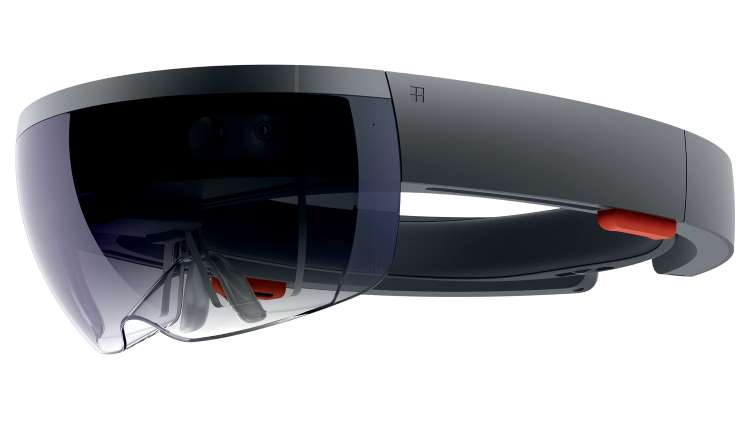
\includegraphics[width=5cm]{Hololens}\label{fig:Hololens}}}%
    \qquad
    \subfloat[Meta 2 \acrshort{acr:AR}-Brille]{{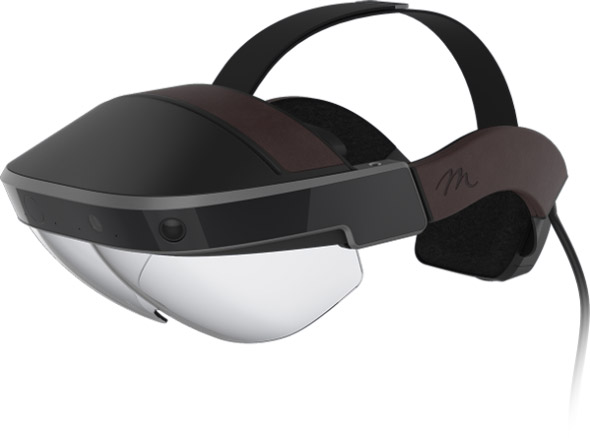
\includegraphics[width=4cm]{Meta2}\label{fig:Meta2}}}%
    \caption{Die zwei potentiellen \acrshort{acr:AR}-Brillen}\label{fig:AR-Brillen}%
\end{figure}

\subsection{\acrshort{acr:VR}-Brillen im Vergleich}
Die, in dieser Arbeit, entwickelte Methode zur \glslink{glos:Labeling}{3D-Datennotation} ist vorwiegend für einen normalen Arbeitsplatz im Büro konzipiert, also einen Platz an dem man einen Desktop-Computer zur Verfügung hat. Deswegen macht es keinen Sinn \acrshort{acr:VR}-Brillen in Betracht zu ziehen die von einem mobilen Gerät betrieben werden (Samsung Gear VR), da diese deutlich weniger Leistung und eine schlechtere Bedienung haben als Geräte für einen Desktop-PC. Auch die Nutzung der Playstation VR ist nicht sinnvoll, da zum Betrieb eine Playstation 4 nötig ist, welche in den wenigsten Unternehmen vorhanden sein dürfte.

Für das \glslink{glos:Labeling}{Klassifizieren} im dreidimensionalen Raum ist eine gute Darstellung und Bedienung notwendig. Bei \acrshort{acr:VR}-Brillen, die einen Desktop-PC als Recheneinheit haben wird beides geboten. Durch die hohe Leistung eines performanten Computers kann der dreidimensionale Raum hochauflösend dargestellt werden. Auch die genaue, für Spiele konzipierte, Steuerung über Controller kommt einem \glslink{glos:Labeling}{Labeling}-Tool zugute. Zum Zeitpunkt der Erstellung dieser Arbeit, gibt es zwei relevante VR-Brillen aus dieser Sparte, die Oculus Rift und die HTC Vive.

\subsubsection{Oculus Rift}
Mit 470 Gramm ist die Oculus Rift (vgl. Abbildung \ref{fig:Oculus}) deutlich leichter als andere Modelle, wie beispielsweise die HTC Vive mit 600 Gramm oder die Playstation VR mit 610 Gramm \cite{bib:OculusTestTragekomfort}. Dies ist für längeres Arbeiten mit ihr sehr vorteilhaft, da schwere Brillen oft schon nach kurzer Zeit störend beim Tragen sind. Des weiteren lässt sich die Brille problemlos an jedem handelsüblichen Büro-Arbeitsplatz verwenden. \textit{\glqq Oculus empfiehlt, die Kameras im Abstand von zwei Metern nebeneinander zu platzieren – bei einem klassischen PC-Arbeitsplatz also links und rechts neben dem Monitor. Das funktioniert in der Praxis gut, man kann sich mit diesem Aufbau ungefähr jeweils einen Schritt in alle Richtungen bewegen\grqq} \cite{bib:OculusTouchTest}. Auch in Sachen Steuerung ist die Oculus Rift anderen Modellen überlegen. Durch die sogenannten Touch Controller, mit denen man virtuell nicht nur Greifen, sondern auch Daumen und Zeigefinger bewegen kann, gelingen ihr \textit{\glqq deutlich feinere Bewegungen\grqq} als beispielsweise der HTC Vive \cite{bib:OculusTouchTest}. Dies bietet für die Entwicklung einer Lösung zur Markierung vieler Objekte zahlreiche Möglichkeiten.\\

Was bei der Oculus Rift nicht so gut funktioniert, wie bei anderen Brillen ist das \gls{glos:Roomscaling}, also das Erfassen der Bewegungen des Benutzers durch einen größeren Raum. Hierfür gibt es bei der Rift zwei Methoden, einmal mit zwei Kameras (kleine Überwachungsfläche) die sich im Abstand von drei Metern in zwei Raumecken gegenüberstehen und eine mit drei Kameras (größere Überwachungsfläche). Beide Methoden funktionieren nicht einwandfrei und auch nicht so gut wie bei der HTC Vive \cite{bib:OculusTouchTest}.

\subsubsection{HTC Vive}
Die HTC Vive (vgl. Abbildung \ref{fig:Vive}) punktet mit dem ausgeklügelten Lighthouse Tracking System, welches in Zusammenarbeit mit VALVE entwickelt wurde \cite{bib:Lighthouse}. Das System kann die Kopfbewegungen des Benutzers durch mehr als 70 Sensoren, welche sowohl in die Brille integriert als auch extra positioniert sind, auf bis zu ein zehntel eines Grades messen \cite{bib:ViveTest}. Auch die Controller werden durch dieses System erfasst, was zu einer genauen Übertragung der physischen Handbewegungen in die virtuelle Welt führt. Dies kommt der Auswahl zahlreicher Objekte, wie es bei der Klassifizierung von Punkten der Fall ist, sehr entgegen. Auch eine gute Darstellung ist dank zweier Displays gewährleistet, die jeweils eine Auflösung von 1080 auf 1200 Pixel haben. Bei diesen Displays kommt es weder zu Verzerrungen des Bildes (\textit{\glqq lens distortion\grqq} \cite{bib:ViveTest}) noch zu Pixelfehlern. Ebenfalls nützlich, vor allem am Arbeitsplatz, ist die Bluetooth-Funktion der Vive. Damit ist es möglich sein Smartphone mit der Brille zu verbinden und somit eingehende Emails oder Ähnliches zu lesen und zu beantworten, ohne die Brille absetzen zu müssen.\\  

Der große Unterschied zwischen Vive und Rift liegt bei der Bedienung durch die unterschiedlichen Controller. Hier hat die HTC-Brille das Nachsehen, weil sie durch Anatomie der Controller weniger Möglichkeiten zur Interaktion in der virtuellen Umgebung bietet. Die sogenannten Wands bieten nämlich keinerlei Funktionen die es ermöglichen eine Hand nachzuahmen, um beispielsweise einzelne Finger zu bewegen und somit virtuelle Objekte greifen zu können. Im Hinblick auf eine durchdachte Steuerung für die Auswahl und Markierung vieler Punkte in einer Punktwolke gibt es somit weniger Möglichkeiten diese zu entwickeln.

\begin{figure}%
    \centering
    \subfloat[HTC Vive \acrshort{acr:AR}-Brille mit Controllern]{{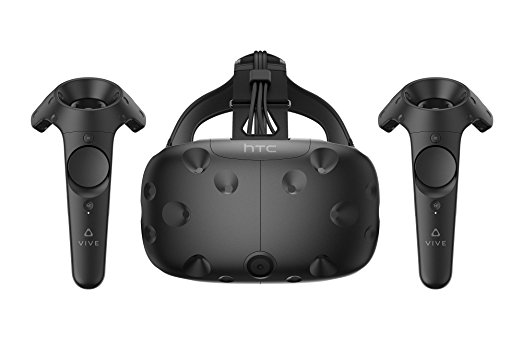
\includegraphics[width=5cm]{Vive}\label{fig:Vive}}}%
    \qquad
    \subfloat[Oculus Rift \acrshort{acr:VR}-Brille mit Controllern]{{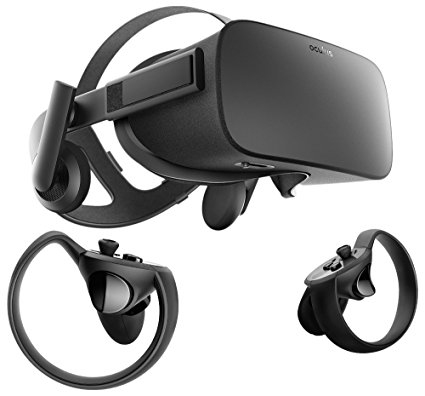
\includegraphics[width=3cm]{Oculus}\label{fig:Oculus}}}%
    \caption{Die zwei potentiellen \acrshort{acr:VR}-Brillen}\label{fig:VR-Brillen}%
\end{figure}

\subsection{Zusammenfassung und Entscheidung}
Für die Wahl des passenden Mediums, auf dem das dreidimensionale \glslink{glos:Labeling}{Labeling} entwickelt werden soll, sind mehrere Faktoren entscheidend. Diese Faktoren ergeben sich danach, wie sehr sich etwas für die genannte Anwendung eignet. Zunächst ist es wichtig eine Punktwolke deutlich und nach Möglichkeit im richtigen Maßstab darzustellen. Hier kommt die \acrlong{acr:AR}-Technologie, durch die Interaktion mit der Umgebung und der lichtempfindlichen Darstellung digitaler Inhalte, sicherlich an ihre Grenzen. In der virtuellen Realität dagegen kann eine solche Wolke problemlos bei jeder Bedingung angezeigt werden, da die reale Umgebung nicht berücksichtigt wird. Sogar der Maßstab kann gut eingehalten werden, da dem virtuellen Raum keine Grenzen gesetzt sind, sodass beliebig große Umfeldmodelle an jedem Arbeitsplatz dargestellt werden können.

Auch die Steuerung spricht für den Einsatz von \acrlong{acr:VR}. Zwar ist das Konzept der Greif-Steuerung der Meta 2 ein guter Ansatz, da diese aber noch nicht zuverlässig und genau funktioniert, ist sie für die Selektion vieler Objekte nicht gut geeignet. Dagegen bietet die Steuerung durch Controller bei \acrshort{acr:VR}-Brillen deutlich mehr Möglichkeiten eine gute Bedienung für das gewünschte Tool zu entwickeln. Die Tasten eines solchen Controllers können vom Entwickler nämlich nach Wunsch programmiert werden wogegen die Gesten für \acrshort{acr:AR}-Brillen nicht verändert bzw. nicht neu erstellt werden sollten \cite{bib:NewGesture}. 

Zudem gibt es, durch die deutlich frühere Markteinführung, viel mehr Dokumentationen und Hilfestellungen im Bereich \acrlong{acr:VR}, was die Entwicklung deutlich erleichtert.

Aufgrund der eben genannten Vorteile von \acrshort{acr:VR} gegenüber \acrshort{acr:AR} wird für die Entwicklung, im Rahmen dieser Arbeit, \textbf{\acrlong{acr:VR}} verwendet.\\

Bleibt noch die Frage zu klären welche Brille verwendet werden soll. Diese Frage ist schwerer zu beantworten als die vorherige. Die zwei potentiellen \acrshort{acr:VR}-Brillen, also Oculus Rift und HTC Vive, sind beide geeignete Kandidaten. Die Vive punktet durch gutes \gls{glos:Roomscaling} und gutes Tracking der Brille und der Controller, wogegen die Oculus Rift guten Tragekomfort und gut durchdachte Controller-Bedienung bietet. 

Wichtig für die Entwicklung einer \glslink{glos:Labeling}{3D-Datennotation} ist aber nicht, ob man sich physisch, also mittels \gls{glos:Roomscaling} durch die Punktwolke bewegen kann, sondern wie man die klassifizierbaren Punkte markieren bzw. auswählen kann. Da hierfür die Oculus Touch Controller mehr Möglichkeiten bieten wird für die Entwicklung eines \acrshort{acr:VR}-\glslink{glos:Labeling}{Labeling}-Tools die \textbf{Oculus Rift} verwendet.    

\section{Wahl des passenden Rechners}
Für die Berechnungen, die notwendig sind um Inhalte in der Oculus anzuzeigen, ist nicht die Brille selbst verantwortlich. Diese Aufgabe übernimmt ein extra Computer. Die Brille fungiert dementsprechend nur als Anzeigegerät. Auch die Sensoren sind an den PC angeschlossen um das Tracking der Brille und der Controller zu gewährleisten. Da vor allem die Grafikberechnungen sehr aufwendig sind, kann nicht jeder handelsübliche PC oder Laptop dazu verwendet werden eine solche \acrshort{acr:VR}-Brille zu betreiben.\\ 

Wichtig sind also zunächst die Basiskomponenten wie ein schneller Prozessor und eine leistungsstarke Grafikkarte. Aber auch ein schneller Arbeitsspeicher mit ausreichender Kapazität ist wichtig damit notwendige Daten so schnell wie möglich zur Verfügung stehen. Für die Wahl, welche Komponenten eingesetzt werden sollen, kann sich an den empfohlenen Spezifikationen des Herstellers orientiert werden (Oculus Rift Recommended System Specs \cite{bib:OculusSpecs}). Diese sind jedoch vorwiegend für den Endnutzer gedacht, bei dem es wichtig ist ein einzelnes Programm für die Brille auszuführen. Für die Entwicklung ist dagegen mehr Leistung notwendig. Soll zum Beispiel eine erstellte Software getestet werden, muss nicht nur die Software selber, sondern eventuell auch die Entwicklungsumgebung und zusätzliche \glslink{glos:Debugger}{Debugging-} und  Analyse-Tools ausgeführt werden. An dieser Stelle sollte also nicht gespart werden.\\

Sind die Basiskomponenten ausgewählt, sollte noch geprüft werden ob noch weiteres Zubehör wichtig ist um diese zu betreiben. Da gerade Prozessoren mit hoher \gls{glos:Taktrate} viel Wärme produzieren, muss stets für ausreichende Kühlung gesorgt werden. Bei der Rechner-Konfiguration für diese Masterarbeit wurden beispielsweise, neben einem hochwertigen Prozessorkühler, noch zwei weitere Gehäuselüfter verbaut, um die Abwärme aus dem inneren des Computers heraus zu leiten. Zu guter Letzt ist es wichtig ein passendes Mainboard auszuwählen, auf dem alle Komponenten verbaut werden. Für die Oculus Rift werden vier USB-Anschlüsse empfohlen, welche das Mainboard haben muss \cite{bib:OculusSpecs}. Ebenfalls muss das Board genug Platz bieten um die gewählten Komponenten zusammen anbringen zu können. Leistungsstarke Grafikkarten und Prozessorlüfter können zum Teil sehr groß ausfallen. Auch für weitere Aufrüstungen sollte das Board genügend Platz bieten, falls es, zu einem späteren Zeitpunkt, notwendig wäre zusätzliche Komponenten (zweite Grafikkarte) hinzuzufügen. Unter Berücksichtigung der eben genannten Aspekte wurde folgende Rechner-Konfiguration für die Entwicklung verwendet:\\  

\begin{table}[h]
 \begin{tabular}{lcr}
  \textbf{Bezeichnung der Komponente} & \textbf{Verwendete Komponente}\\
  \\
  
  \textit{Prozessor:} & Intel® Core™ i7-7700K\\
  \textit{Grafikkarte:} & Gainward GeForce GTX 1070 Phoenix\\
  \textit{Mainboard:} & ASUS PRIME Z270-A\\
  \textit{Arbeitsspeicher(RAM):} & HyperX DIMM 16 GB DDR4-2400 Kit\\
  \textit{Festplatte:} & Samsung 850 Pro 2,5"\ 512 GB\\
  \textit{Netzteil:} & Cooler Master G550M 550W\\
  \textit{Prozessorlüfter:} & Noctua NH-D9L\\
  \textit{Gehäuselüfter:} & 2x Coolink SWiF2-1200 120x120x25\\
  \textit{Gehäuse:} & Cooler Master N300\\
\\
 \end{tabular}
 \caption{Rechner-Konfiguration für die Entwicklungen dieser Arbeit}
 \label{tab:Rechnerkonfig}
 \end{table}

\section{Wahl der passenden Entwicklungsplattform}
Für die Erstellung von \acrlong{acr:VR} Software gibt es zwei Entwicklungsumgebungen, die gut für das Entwickeln von \acrlong{acr:VR} geeignet sind, weil sie schon seit längerem \acrshort{acr:VR}-Support bieten und dies auf umfassende Weise. Diese sind  Unreal Engine 4 und Unity Engine. Beide Plattformen bieten alles nötige um \acrshort{acr:VR}-Software zu entwickeln, weshalb die Wahl zwischen ihnen eher subjektiv, aufgrund der eigenen Bedürfnisse und Erfahrungen, zu fällen ist. 

Im Allgemeinen kann man sagen, dass die Unreal Engine mehr Möglichkeiten für professionelles Game Engineering bietet, da viel Wert auf visuelle Qualität gelegt wird, beispielsweise durch integrierte \gls{glos:PostPr}-Techniken und bessere \gls{glos:Shader}. Sie bietet neben dem \gls{glos:Scripting} auch die Gelegenheit, durch C++ Programmierung Module der Engine zu verändern bzw. neue hinzuzufügen. Das gestalten von \glspl{glos:UI} ist mit dem UMG UI Designer ebenfalls gut gelöst \cite{bib:UEvsUE4}.

Die Unity Engine bietet vor allem Anfängern einen leichten Einstieg in die Welt der Grafik- und Spieleprogrammierung. Im Editor können ganz einfach sogenannte Game Objects erstellt werden, denen dann Funktionalitäten und Eigenschaften angehängt werden können. Dies geschieht meist in Form von Skripten, welche oft schon vorgefertigt zur Verfügung stehen. Wenn dies nicht der Fall ist können diese angepasst oder neu erstellt werden. Die große Community der Unity Engine ist hierbei eine große Hilfe.

\subsubsection{Entscheidung}
Ein Vorteil den die Unity Engine, im Falle dieser Arbeit, bietet ist Nutzung von C\# als \gls{glos:Scripting}-Sprache. Da  
C.LABEL (vgl. \ref{sec:C.LABEL}) ebenfalls in C\# programmiert wurde können Komponenten, wie etwa das Einlesen von Daten in die Anwendung, leicht übernommen werden. Des Weiteren habe ich selbst schon, im Rahmen eines Universitätsprojekts, mit dieser Engine gearbeitet, weshalb ein längeres einarbeiten in die Entwicklungsumgebung nicht nötig wäre. Die Vorteile der Unreal Engine sind, wie schon erwähnt, die visuelle Präsentation und die dabei gebotene Performance. Diese sind vor allem für das erstellen aufwändiger Landschaften und deren Inhalten von Vorteil. 

Für die Entwicklung der, in dieser Arbeit, angestrebten Anwendung spielen jedoch Dinge wie Grafik und beeindruckendes Leveldesign keine große Rolle. Viel wichtiger ist sowohl die Möglichkeit der Kompatibilität zur C.LABEL-Anwendung als auch die vorhandene Entwicklungserfahrung einer Engine. Gerade letzteres ist auf Grund des begrenzten Zeitrahmens einer Masterarbeit von Vorteil, da ohne große Einarbeitung mehr Zeit zum Entwickeln von Funktionalität und Optimierungen bleibt. Aus diesen Gründen wird im weiteren Verlauf dieser Arbeit die \textbf{Unity Engine} als Entwicklungsumgebung verwendet.












\chapter{Grundlagen}
\graphicspath{{Kapitel/Kapitel2_Grundlagen/Images/}}

%Dieses Kapitel befasst sich mit einigen grundlegenden Themen, die mit dem Inhalt dieser Arbeit zu tun haben. Dies soll dem besseren Verständnis für die folgenden Kapitel dienen. Der Abschnitt \ref{sec:MLearning} beispielsweise, befasst sich mit dem Prinzip des maschinellen Lernens auf Basis von neuronalen Netzen, was verdeutlichen soll warum die Daten der Punktwolken überhaupt \glslink{glos:Labeling}{gelabelt} werden müssen. Anschließend wird die CMORE Inhouse Software C.LABEL in \ref{sec:C.LABEL} vorgestellt um den aktuellen Stand der Technik im Bereich Punktwolkenannotierung zu zeigen. \ref{sec:UnityEngine} stellt die \gls{glos:GameEngine} Unity vor, die benutzt wurde um die \acrlong{acr:VR} Applikation zu erstellen.

\section{Annotation}
\label{sec:Annotation}
warum?
was für arten?

\subsection{Maschinelles Lernen}
\label{sec:MLearning}
Der Ausdruck Maschinelles Lernen (engl.: \textit{Machine Learning}) ist heutzutage ein Überbegriff für Methoden, die versuchen durch Optimierung eine Funktion zu erlernen. Bei solch einer Funktion kann es sich sowohl um eine simple binäre Entscheidung auf eine Fragestellung handeln als auch um komplexere Dinge wie das Übersetzen von Texten in eine andere Sprache, das Erkennen von Personen auf Bildern, oder eben das Klassifizieren von Objekten in einer Punktwolke. Letzteres ist speziell für diese Arbeit relevant. Die Komplexität der Funktion bestimmt auch die zu verwendende Methode zur Lösung des Problems. Im Zuge des \textit{Azure Machine Learning Studios} veröffentlichte Microsoft eine Graphik (vgl. Abbildung \ref{fig:MLCS}), mit der man den richtigen Lernalgorithmus für gewisse Vorhersage-Methoden bestimmen kann. Für die Objektklassifizierung im Automobilbereich ist es wichtig die Klasse eines Objekts mit hoher Genauigkeit aus einer großen Anzahl verschiedener Klassen zu bestimmen. Basierend auf der Graphik \ref{fig:MLCS} ist die beste Methode dafür die Verwendung eines künstlichen neuronalen Netzes(\acrshort{acr:knn}). Die Benutzung solcher Netze ist üblich, wenn es um Klassifikation von vielen verschiedenen Dingen geht und soll im Folgenden näher erläutert werden.\\

TODO Grafik von Bild und wolkenerkennung\\

\begin{figure}%
	\centering
    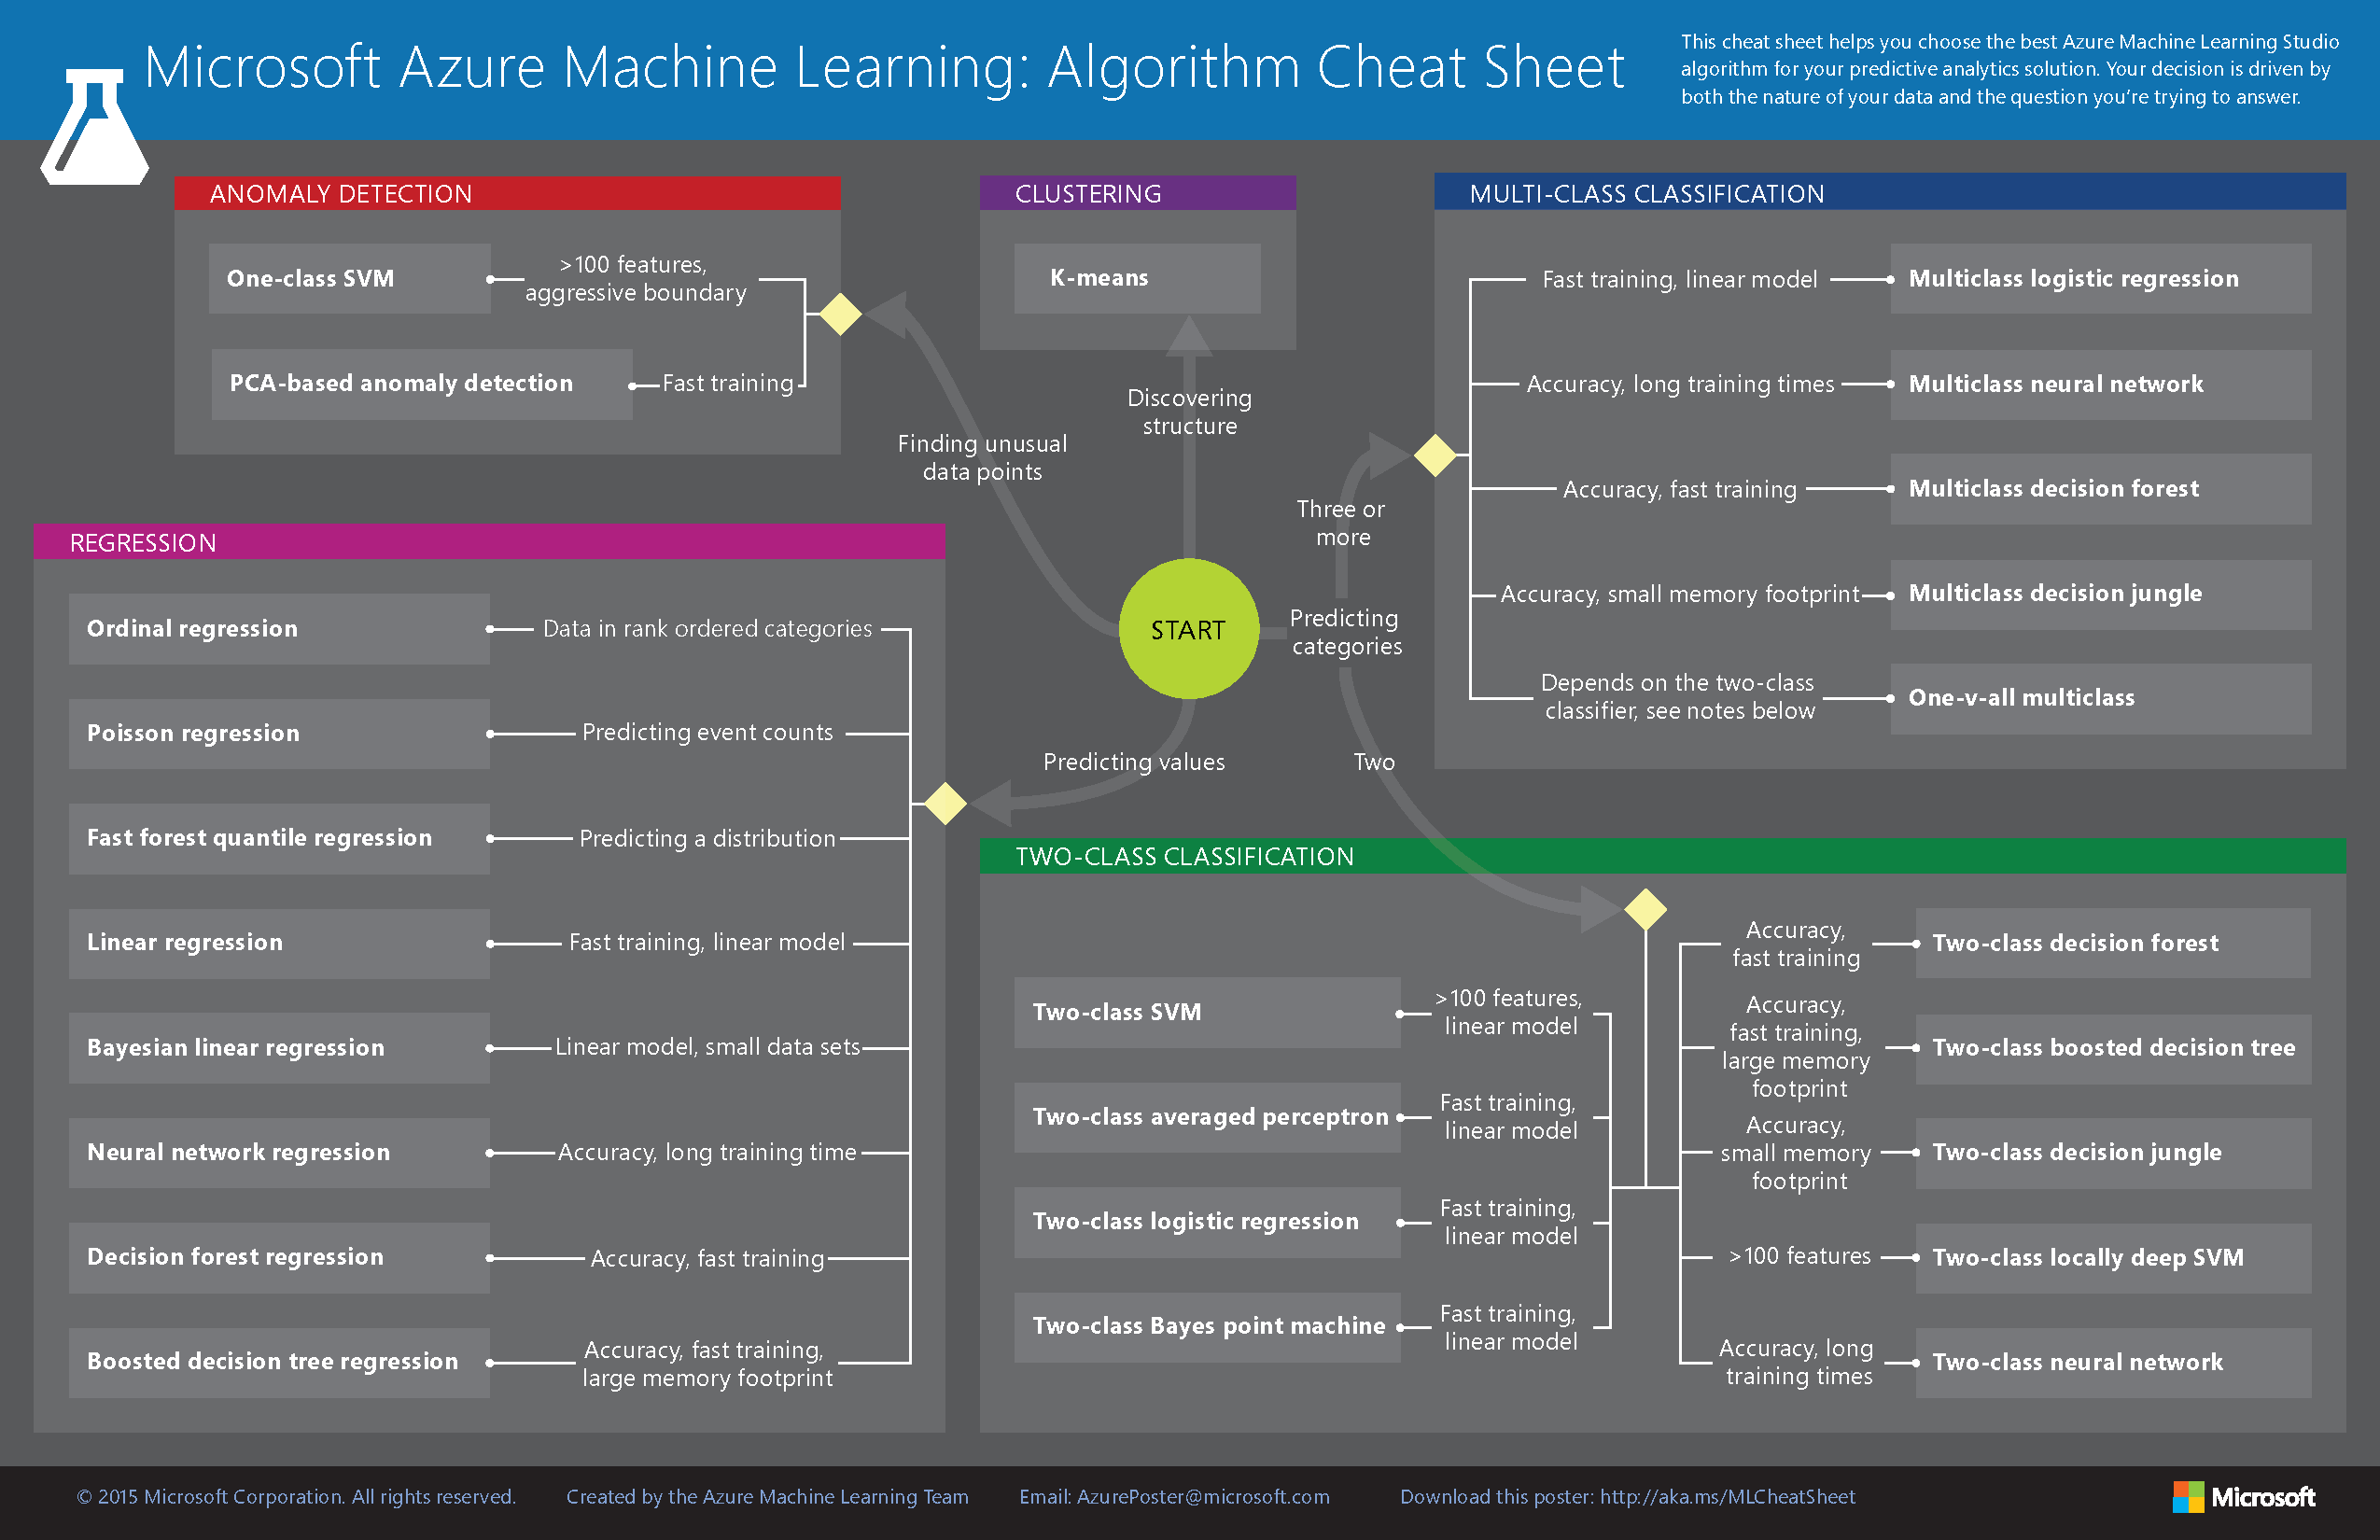
\includegraphics[width=19cm, angle=270]{MLCS}
    \caption{Diagramm um den besten Machine Learning Algorithmus für eine \gls{glos:PredAna}-Methoden zu finden \cite{bib:AzureCs}}
    \label{fig:MLCS}
\end{figure}
  
\subsubsection{Künstliche Neuronale Netze}
\label{sec:KNN}
David Kriesel hat in \cite{bib:UebereblickNN} den Zusammenhang zwischen physischen und künstlichen neuronalen Netzen dargestellt. Seine Arbeit soll im Folgenden als Quelle dienen. Das Prinzip der künstlichen neuronalen Netze ist, wie vieles in der Informatik, einer Struktur aus der realen Welt nachempfunden. Das komplexeste neuronale Netz ist wohl das menschliche Gehirn mit etwa 86 Milliarden Nervenzellen, welche auch Neuronen genannt werden. Daher kommt auch der Begriff des neuronalen Netzes. Diese Nervenzellen sind durch Synapsen mit bis zu mehreren Tausend anderen Zellen verbunden. Diese Verbindungen bilden zusammen das Netz. Die Kommunikation zwischen den Neuronen erfolgt in der Regel über elektrische Impulse und chemische Botenstoffe. Beides wird über Synapsen zu den nächsten, verbundenen Neuronen weitergeleitet und bewirkt dort einen Reiz. Durch Übertragung von chemischen Botenstoffen kann dieser Reiz zusätzlich gewichtet werden, das heißt es kann ein stärkerer oder schwächerer Reiz ausgesendet werden. Alle ankommenden Reize werden dann am Empfangsneuron akkumuliert und ergeben den Eingangsreiz des Neurons.\\ 

Dieses, vereinfacht dargestellte Prinzip, wird auch bei den  \acrshort{acr:knn}s verwendet. Übersteigt dieser Reiz eine bestimmte Schwelle kommt es zum entscheidenden Ereignis: Das Neuron \textit{feuert}. Dadurch gibt das feuernde Neurone einen Impuls an alle anderen Neuronen weiter mit dem es verbunden ist. Bei dafür vorgesehenen Neuronen oder verbänden davon, kann dieser Impuls auch ein Ereignis auslösen. Diese Ereignisse können physischer Natur sein, also beispielsweise Bewegungen, oder auch psychischer Natur, zum Beispiel das Erkennen von Dingen. Werden diese Nervenzellen also mit einem ausreichenden Impuls angesprochen, wird das entsprechende Ereignis ausgelöst.\\

\begin{figure}%
	\centering
    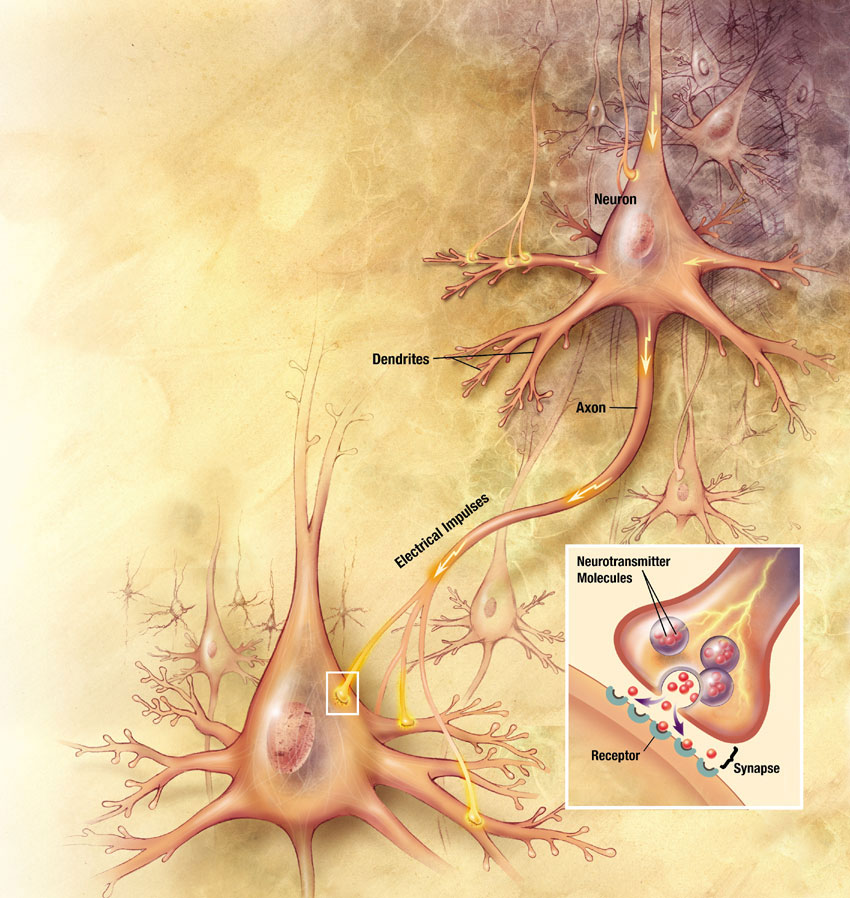
\includegraphics[width=9cm]{Neurons}
    \caption{Abbildung des Übertragungsprinzips von Reizen zwischen Neuronen \cite{bib:Neurons}}
    \label{fig:MLCS}
\end{figure}

Die entscheidende Komponente dieses Prinzips ist die adaptive Gewichtung der weitergegebenen Reize. Adaptiv deswegen, da die Gewichtung der Reize sich während eines Menschenlebens verändern können. So erkennen Kinder oft Gefahrensituation nicht, da ihr Gehirn nicht ausreichend geschult ist um diese zu erkennen. In diesem Kontext bedeutet das, dass an die \textit{Gefahren-Neuronen} kein ausreichend starker Reiz gesendet wird. Durch sammeln von Erfahrungen optimiert sich dieser Wert, was in späteren Jahren zu einer anderen Reaktion des Gehirns führen kann als früher. Das Adaptieren dieser Gewichte auf einen passenden Wert bezeichnen wir als Lernen. Um Computersystemen einen derartigen Lerneffekt zu ermöglichen wurde dieses Biologische Prinzip nun mathematisch imitiert. \\

\begin{figure}%
	\centering
    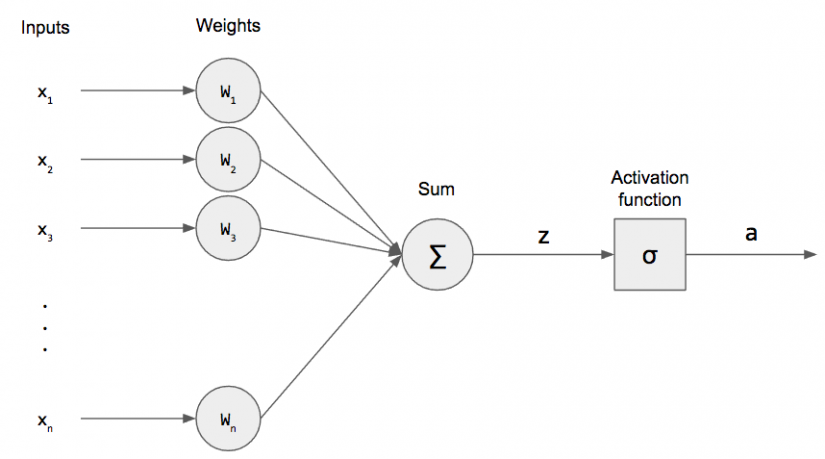
\includegraphics[width=13cm]{Perceptron}
    \caption{Einfaches Perzeptron nach dem Prinzip von Frank Rosenblatt}
    \label{fig:Perceptron}
\end{figure}

Künstliche Neuronale Netze basieren auf dem Prinzip des Perzeptrons, das von Frank Rosenblatt 1958 vorgestellt wurde \cite{bib:Perzeptron}. Dieses Perzeptron repräsentiert die Funktion eines einzelnen Neurons auf eine mathematische Weise (vgl. \ref{fig:Perceptron}). Die Eingangsdaten eines Perzeptrons bestehen aus einer \(n\)-großen Menge an Werten \(x_1 \dots x_n\), welche eine gleichgroße Menge an jeweiligen Gewichten \(W_1 \dots W_n\) haben. Wenn das zu analysierende Ziel beispielsweise ein Bild ist, wäre \(n\) die Menge aller Pixel des Bildes und bei Punktwolken eben die Anzahl der Punkte. Die Eingangswerte werden von einer mathematischen Funktion empfangen und zu einem skalaren Wert \(z\) zusammengefasst. Hierbei wird meist die Gewichtete Summe benutzt die folgendermaßen berechnet wird:

\begin{equation}
z = \sum \limits_{i=0}^{n} W_i \cdot x_i
\end{equation}\\

Im biologischen Vorbild repräsentiert diese Summe den eingehenden Reiz in eine Nervenzelle, die \(x\)-Werte sind dabei die Impulse der vorherigen Neuronen und die \(W\)-Werte repräsentieren die Gewichtung, also die Stärke der Eingangsreize. Der biologische Schwellwert wird im Perzeptron durch eine Mathematische Funktion \(\sigma(z)\) dargestellt. Wie in \cite{bib:NeuronaleNetze} beschrieben gibt es dafür zwei beliebte Funktionen. Die \textit{Fermifunktion} (\ref{eq:Fermi}) , auch Logische Funktion genannt, welche einen Ausgabe-Wertebereich von (0,1) hat und den \textit{Tangens Hyperbolicus} (\(tanh(z)\)) mit einem Wertebereich von (-1,1). Beide sind differenzierbar, was wichtig für das Lernen mit \textit{Backpropagation} ist. Was das bedeutet wird in Abschnitt \ref{sec:Training} näher erläutert. Wenn der Wert, den diese Funktion liefert, nicht noch durch eine weitere Ausgangsfunktion verändert wird, ist er der Ausgangswert des Perzeptrons.

\begin{equation}
\sigma(z) = \frac{1}{1 + e^{-z}}
\label{eq:Fermi}
\end{equation}

In \acrshort{acr:knn}s können mehrere dieser Perzeptrons eine sogenannte Schicht bilden. Je mehr Schichten ein neuronales Netz hat desto \textit{tiefer} ist es, daher auch der Begriff \textit{Deep Learning}, also tiefes Lernen. In der Regel bestehen \acrshort{acr:knn}s aus mindestens 3 Schichten, nämlich einer Eingangsschicht, einer oder mehrerer Zwischenschichten und einer Ausgangsschicht (veranschaulicht in Abbildung \ref{fig:Bilderkennung}). Die einzelnen Schichten werden im Folgenden kurz erläutert.  

\begin{itemize}
\item \textbf{Eingangsschicht}\\
Die Eingabeschicht ist der Startpunkt des Informationsflusses in einem künstlichen neuronalen Netzes. Eingangssignale werden von den Neuronen dieser Schicht aufgenommen und gewichtet an alle Neuronen der ersten Zwischenschicht weitergegeben. Die Anzahl der Neuronen dieser Schicht hängt, wie schon erwähnt, von den Eingangsdaten ab. Werden Bilder mit einer Auflösung von 50x50 Pixeln in das Netz gespeist, hat dieses Netz in der Regel 50x50, also 2500 Neuronen in der Eingangsschicht.

\item \textbf{Zwischenschicht}\\
Zwischen der Eingabe- und der Ausgabeschicht befindet sich in jedem künstlichen neuronalen Netz mindestens eine Zwischenschicht, die auch verborgene Schicht (engl.: \textit{hidden layer}) genannt wird. Theoretisch ist die Anzahl der möglichen verborgenen Schichten in einem künstlichen neuronalen Netzwerk unbegrenzt. In der Praxis bewirkt jede hinzukommende Schicht jedoch auch einen Anstieg der benötigten Rechenleistung, die für den Betrieb des Netzes notwendig ist.

\item \textbf{Ausgangsschicht}\\
Die Ausgabeschicht liegt hinter den Zwischenschichten und bildet die letzte Schicht in einem künstlichen neuronalen Netz. In der Ausgabeschicht angeordnete Neuronen sind jeweils mit allen Neuronen der letzten Zwischenschicht verbunden. Die Ausgabeschicht stellt den Endpunkt des Informationsflusses in einem \acrshort{acr:knn} dar und enthält das Ergebnis der Informationsverarbeitung durch das Netzwerk. Beim Beispiel der Objektklassifikation besteht die Ausgabeschicht nun aus \(n\) vielen Endknoten, wobei \(n\) die Menge an möglichen Klassifikationen ist. Die Eingangssumme dieser Knoten, den sie aus den vorherigen Neuronen bekommen, entsprechen der Wahrscheinlichkeit, dass es sich bei den Eingangsdaten um die jeweilige Klasse handelt. Abbildung \ref{fig:Bilderkennung} soll dieses Prinzip veranschaulichen.
\end{itemize}

\begin{figure}%
	\centering
    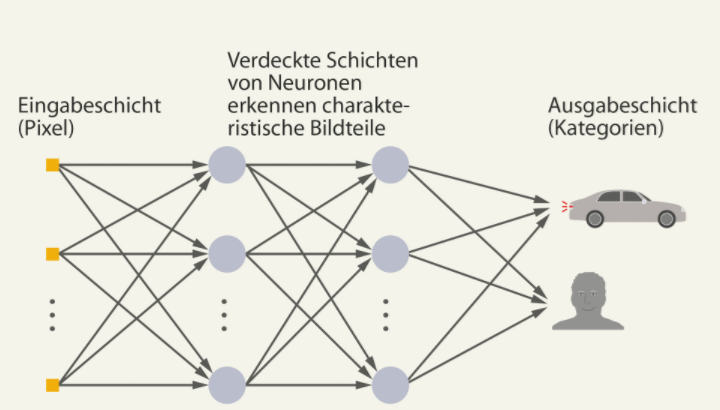
\includegraphics[width=13cm]{Bilderkennung}
    \caption{Stark vereinfachte Darstellung eines \acrshort{acr:knn}s zur Erkennung von Autos und Personen}
    \label{fig:Bilderkennung}
\end{figure}

\subsubsection{Trainieren von künstlichen neuronalen Netzen}
\label{sec:Training}

Damit ein Mensch eine neue Tätigkeit beherrscht muss er diese erst erlernen. In der Regel muss diese Tätigkeit dafür so oft es geht geübt werden. Bei künstlichen neuronalen Netzen ist das genauso. Das Üben bezeichnet man in diesem Kontext als \textit{Trainieren} von Netzen. Im allgemeinen bedeutet der Vorgang des Lernens, dass ein System sich in irgendeiner Form verändert, um sich z.B. an Veränderungen in seiner Umwelt anzupassen. Die typische Veränderung von künstlichen neuronalen Netzen ist das adaptieren der Verbindungsgewichte \(W_1 \dots W_n\). Damit die Verbindungsgewichte auf einen passenden Wert verändert werden muss das Netz entsprechend oft trainiert werden. Dies geschieht nach Regeln, die man in Algorithmen definiert – ein Lernverfahren ist also immer ein Algorithmus, den man einfach mithilfe einer Programmiersprache implementieren kann. Diese Algorithmen lassen sich grob in 3 verschieden Arten einteilen:

\begin{itemize}
\item Unüberwachtes Lernen (\textit{Unsupervised Learning})
\item Bestärkendes Lernen (\textit{Reinforcement Learning})
\item Überwachtes Lernen (\textit{Supervised Learning})
\end{itemize}

Für Objektklassifizierung wird in der Regel das überwachte Lernen verwendet, darum wird im Folgenden nur auf das dieses Verfahren eingegangen.\\
 
Der Lernprozess bei dieser Methode ist, wie der Name schon sagt, überwacht. Das kommt daher, dass der Mensch eine Menge an selbst ausgewählten Trainingsbeispielen erstellt. Das wird dann mit dieser überwachten Menge trainiert. Die Trainingsbeispiele bestehen aus eine Menge \(P\) an Eingabemustern mit jeweiliger korrekter Lösung. Das Netz kann seine eigene Ausgabe mit der richtigen Lösung des Beispiels vergleichen und somit eine Fehlerbeschreibung zurückgeben. Für das Beispiel der Punktwolkenklassifizierung bestünde dabei das Trainingsset aus vielen verschiedenen Punktwolken, die alle ein Objekt darstellen, wobei die Art des Objektes, also die Lösung der Klassifizierung, bekannt ist. \\

Die Werte der Gewichte \(W_1 \dots W_n\) werden bei einem untrainierten Netz zu Beginn zufällig gewählt. Dadurch gibt ein solches Netz in der Regel völlig falsche Lösungen für die ersten Trainingsbeispiele aus. Das ist aber nicht weiter schlimm, da nun der Lerneffekt einsetzen soll. Durch die Bekanntheit der Lösung des Beispiels kann der Fehler zwischen dem Ergebnis des Netzes und der gewünschten Lösung genau bestimmt werden. Dieser Fehler kann anschließend durch zurückrechnen auf jedes Neuron der vorherigen Schichten projiziert werden. Auf diese Weise kann der Fehler, den jedes einzelne Neuron verursacht bestimmt werden. Dieses Zurückrechnen nennt sich \textit{Backpropagation}. Aus dem Fehler den jedes Neuron verursacht kann schließlich der Betrag errechnet werden, um den sich das Gewicht \(W_i\) des Neurons verändern muss, damit bei zukünftigen Eingaben bessere Ergebnisse erzielt werden. Für das Verständnis des Grundprinzips ist die Formel zu Berechnung der Gewichtsänderung nicht wichtig, sie wird aber zur Vervollständigung im Folgenden angegeben: 

\begin{equation}
\triangle w_{ij} = -\eta\delta_jo_i
\label{eq:BackProb}
\end{equation}

\begin{itemize}
\item \(\triangle w_{ij}\) ist die Änderung des Gewichts \(w_{ij}\) der Verbindung von Neuron \(i\) zu Neuron \(j\)
\item \(\eta\)  ist ein fester Wert, der eine Lernrate ausdrücken soll, mit der die Stärke der Gewichtsveränderung festgelegt wird
\item \(\delta_j\) ist das Fehlersignal des Neurons \(j\) das sich aus der partiellen Ableitung \(\frac{\partial E}{\partial net_j}\) ergibt\\
\begin{itemize}
\item \(E\) ist dabei der quadratische Fehler der bei der Berechnung des Ergebnisses entstand, er wird durch die Formel \(E = \sum \limits_{i=1}^n (t_i - o_i)^2\) berechnet
\begin{itemize}
\item \(t_i\) steht darin für den gewünschten Zielwert
\end{itemize}
\item \(net_j\) ist die Netzeingabe \(\sum \limits_{i=1}^n x_iw_{ij}\)
\end{itemize}

\item \(o_i\) steht sowohl bei der Berechnung von \(\triangle w_{ij}\), als auch von \(E\) für die errechnete Ausgabe des Neurons \(i\)
\end{itemize}

Zusammenfassend kann man nun sagen, dass der Lernprozess eines künstlichen Neuronalen Netzes nach folgendem Schema abläuft:

\begin{enumerate}
\item \textbf{Eingabe} eines Elements \(p\) aus der Trainingsmenge \(P\) in die Eingabeschicht des Netzes
\item \textbf{Vorwärtspropagierung} der Eingabe durch das Netz gesamte Netz, sodass man bei der Ausgabeschicht ein Ergebnis erhält
\item \textbf{Vergleich} des Ergebnisses mit der richtigen Lösung und Berechnung des Fehlers
\item \textbf{Zurückpropagieren} des Fehlers, um somit die Gewichte der Neuronen anzupassen
\end{enumerate}

Wie unschwer zu erkennen ist basiert der Backpropagation-Algorithmus auf dem Vorhandensein eines Trainingsdatensatzes. Damit das Netz nach dem Training für neue, unbekannte Eingaben die richtige Lösung errechnet ist es elementar wichtig, dass dieser Datensatz eine hohe Qualität und Quantität hat. Qualität bedeutet in diesem Fall, dass die Trainingsdaten repräsentativ für den jeweiligen Anwendungsfall sein müssen. Ein Personenerkennungsalgorithmus der im Straßenverkehr Personen identifizieren soll liefert keine guten Ergebnisse, wenn er ausschließlich mit Bildern von Personen in Innenräumen gefüttert wird. Mit Quantität ist Anzahl der verschiedenen Elemente im Trainingssatz gemeint. \acrshort{acr:knn}s verbessern ihre Ausgabe in der Regel mit größerer Menge an unterschiedlichen Trainingsdaten.\\

Zur Erstellung dieses Datensatzes ist es nun nötig so viele repräsentative Daten wie möglich zu sammeln und diese mit der richtigen Lösung zu annotieren. Eine Methode für eine solche Annotierung wird in dieser Arbeit vorgestellt. Dieses Kapitel sollte nun veranschaulicht haben warum  solche Methoden so essentiell sind, um künstliche Intelligenzen zu entwickeln.


\section{Virtual Reality}
\label{sec:VirtualReality}

Das Konzept digitale Inhalte räumlich und interaktiv darzustellen ist nicht neu. Die Ursprünge von VR lassen bis 1965 zurückverfolgen als Ivan Sutherland \glqq \textit{The Ultimate Display}\grqq \cite{bib:UltimateDisplay} vorstellte. Diese Arbeit stellte die ersten Konzepte für Immersio̱n in einer virtuellen Welt und die dafür nötigen Ein- und Ausgabegeräte dar. Er wollte damit einen Anreiz schaffen um die Grenzen der damaligen Mensch-Computer-Schnittstelle zu überwinden und neue Applikationen zu entwickeln, welche die eigene Präsenz in der virtuellen Welt miteinbeziehen \cite{bib:VRReport}.\\

Anfang der achtziger Jahre gab es dann schon funktionierende VR-Systeme, beispielsweise das VIVED System (\textit{Virtual Visual Environment Display}), welches von der NASA entwickelt wurde \cite{bib:NasaVr}. Dieses System beinhaltete eine, am Kopf befestigte Brille, mit einem integrierten 2,7\dq{} großen LCD-Display (Abbildung \ref{fig:FirstVrConcept}). Durch Weitwinkelobjektive wird das Bild dieses Displays auf jedes Auge einzeln projiziert. Damit war es möglich Objekte, die normalerweise an einem offenen Bildschirm angezeigt werden, in einer geschlossenen und 3D-ähnlichen Sicht darzustellen (Abbildung \ref{fig:FirstVrUserView}). 

Die Projizierung auf jedes Auge vermittelt dabei einen räumlichen Eindruck, der durch das Prinzip der Stereoskopie verursacht wird \cite{bib:Stereoscopy}. Dieses Prinzip beruht darauf, dass durch zwei Augen die Umgebung aus zwei verschiedenen Blickwinkeln wahrgenommen wird. Dies kann leicht selbst festgestellt werden, indem man einen Finger zwischen die Augen hält und abwechselnd jedes Auge einzeln öffnet. Dabei ist zu erkennen, dass der Finger sich weiter rechts oder links im Blickfeld befindet, je nachdem welches Auge geöffnet ist. Durch die Zusammensetzung der zwei Blickwinkel durch das Gehirn entsteht ein für uns ein Tiefeneffekt. Dieser Effekt wird auch von VR-Brillen genutzt um 2D-Inhalte räumlich wirken zu lassen.

Als Eingabegerät wurde sowohl eine Spracherkennung, als auch ein Handschuh benutzt, der Bewegungssensoren an jedem Finger hatte. Somit war es dem Benutzer möglich auf eine intuitive Weise mit dem System zu Interagieren (Abbildung \ref{fig:FirstVrOutsideView}), da das System die Bewegungen des Benutzers erkannte.\\

Am Prinzip der VR-Technologie hat sich bis heute nicht viel verändert. Die Präsentation der virtuellen Welt geschieht immer noch durch eine Brille mit integrierten Linsen und einem Display (Abbildung \ref{fig:RiftConstruction}). Diese beinhaltet, ebenso wie die Eingabegeräte, Bewegungssensoren, die die Position und Orientierung dieser Komponenten misst.\\ 

\begin{figure}%
    \centering
    \subfloat[VIVED Displayaufbau]{{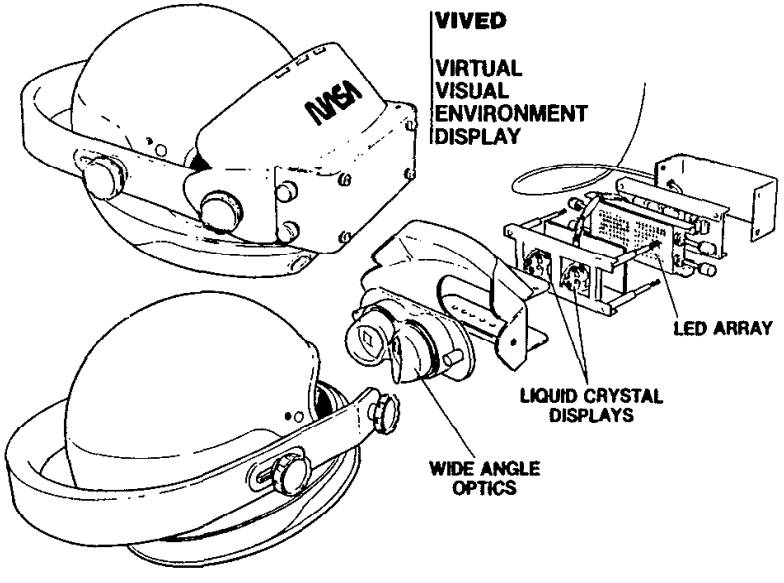
\includegraphics[width=4cm]{FirstVrConcept}\label{fig:FirstVrConcept}}}%
    \qquad
    \subfloat[Sicht eines VIVED Benutzers]{{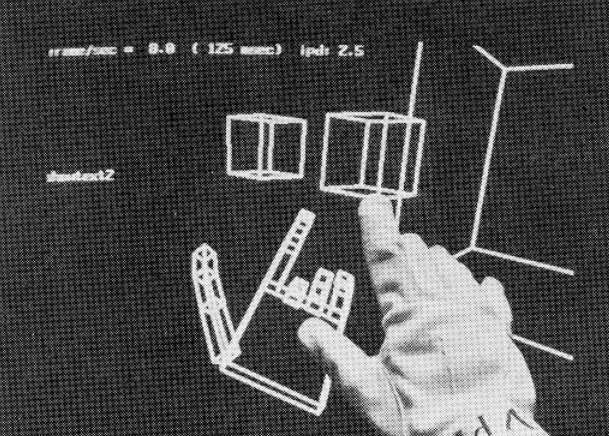
\includegraphics[width=4cm]{FirstVrUserView}\label{fig:FirstVrUserView}}}%
    \qquad
    \subfloat[Sicht auf einen VIVED Benutzer]{{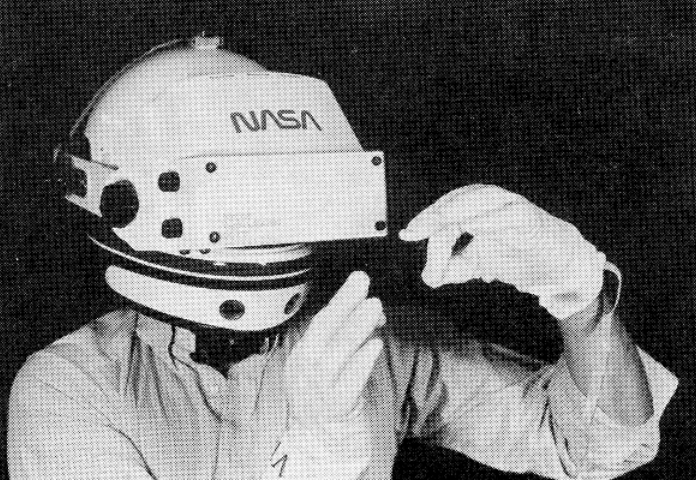
\includegraphics[width=4cm]{FirstVrOutsideView}\label{fig:FirstVrOutsideView}}}%
    \qquad
    \subfloat[Rift Displayaufbau]{{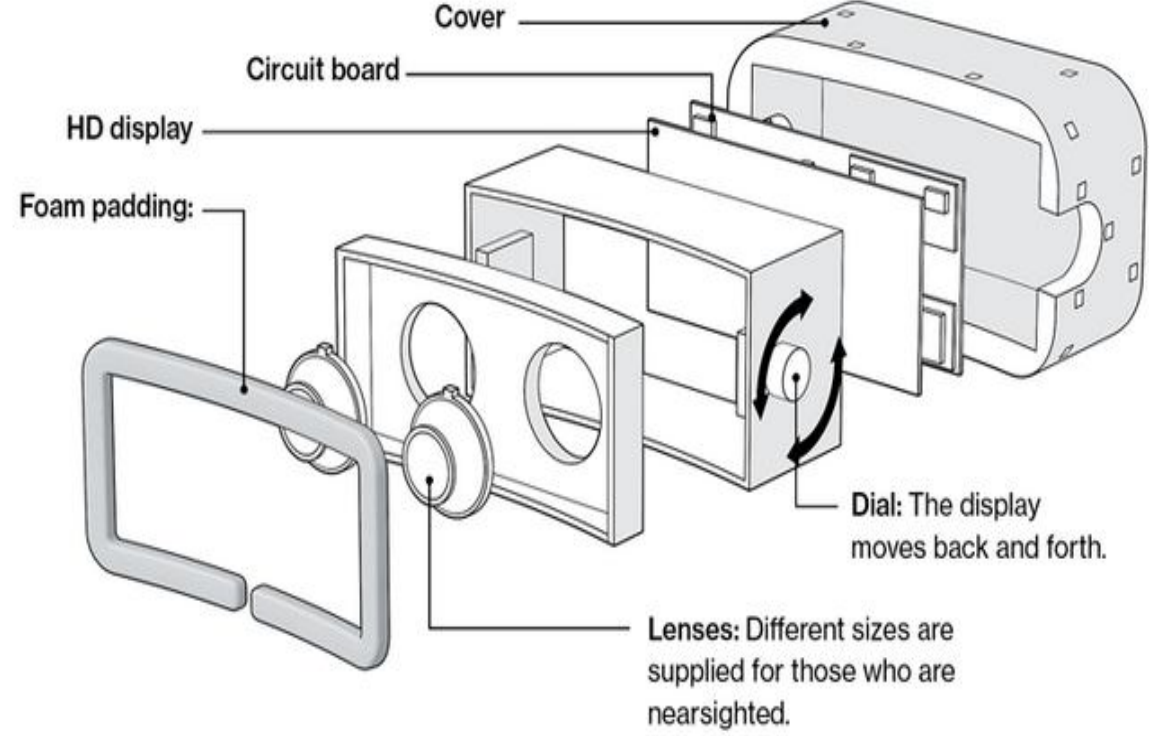
\includegraphics[width=4cm]{RiftConstruction}\label{fig:RiftConstruction}}}%
    \qquad
    \subfloat[Sicht auf einen Rift Benutzer]{{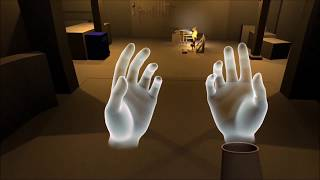
\includegraphics[width=4cm]{RiftAvatar}\label{fig:RiftAvatar}}}%
    \qquad
    \subfloat[Sicht eines Rift Benutzers]{{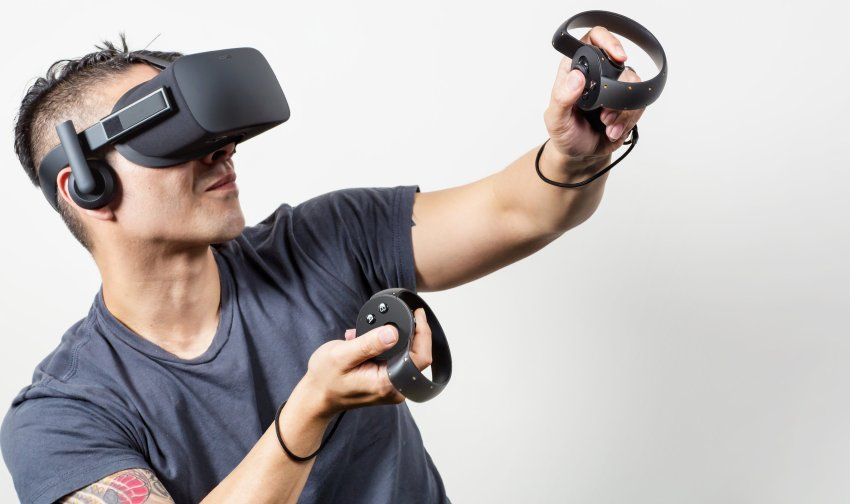
\includegraphics[width=4cm]{RiftUser}\label{fig:RiftUser}}}%
    \caption{Vergleich zwischen den Anfängen der VR-Technologie und dem heutigen Stand. Die oberen drei Bilder zeigen das VIVED-System, das von S.S. Fisher vorgestellt wurde \cite{bib:NasaVr}. Die Unteren zeigen Bilder der Oculus Rift.}\label{fig:VIVED}%
\end{figure}

Die funktionelle Leistung der Komponenten ist im Laufe der Zeit jedoch deutlich besser geworden. Statt eckigen Polygonen können nun hochauflösende 3D-Modelle durch ein Display mit 2160 x 1200 Pixeln dargestellt werden (Abbildung \ref{fig:RiftAvatar}). Die Brille und die Eingabegeräte werden nun auch, zusätzlich zu den internen Bewegungssensoren, von externen Infrarot-Sensoren erfasst, um eine präzise Portierung der physischen Bewegungen in virtuelle zu übersetzen. Der größte Unterschied ist wohl, dass die VR-Technologie heutzutage hauptsächlich für Unterhaltungszwecke genutzt wird. Was früher mal ein Forschungsprojekt einer Raumfahrtorganisation war ist heute ein Entertainment-System, das in viele Privathaushalten zu finden ist.\\

Ein Grund dafür war die Entwicklung der zwei, derzeit geläufigsten VR-Brillen \textit{Oculus Rift} und \textit{HTC Vive}. Ein paar geschichtliche Eckdaten davon wurden in \cite{bib:RiftHistorical} gesammelt. 2010 wurde der erste Prototyp der Oculus Rift von Palmer Luckily entworfen. Dieser hatte eine horizontale Sichtweite von 90°, was zur damaligen Zeit im Verbrauchermarkt einzigartig war. 2013 hatte Valve einen Durchbruch bei der Entwicklung von \textit{Low-Persistence}-Displays, den sie öffentlich geteilt haben. Dies war sehr hilfreich für alle Entwickler, denn Oculus beispielsweise benutzte seitdem bei all ihren nachfolgenden Brillen. Low-Persistence (zu deutsch: \textit{geringe Ausdauer}) bedeutet in dem Falle die angezeigten Bilder nur wenige Millisekunden anzuzeigen um somit Objekte, die sich Bewegen schärfer darstellen zu können. 2014 wurde Oculus Rift für zwei Milliarden Dollar von Facebook gekauft und beschäftigen mittlerweile circa 400 Mitarbeiter allein für die Virtual Reality Entwicklung. Daran kann man das Potential sehen, das große Konzerne in der VR-Technologie sehen, denn kurz danach kündigte nämlich auch Sony eine VR-Brille für die Playstation 4 an.\\

Die, aus der Großproduktion der führenden VR-Konzerne resultierende, Massentauglichkeit und die Erschwinglichkeit der Technologie machen diese aber auch für die Industrie interessant. Vor allem Im Zuge der \textit{Industrie 4.0} ist VR für Digitalisierung des industriellen Umfelds von Nutzen. Es werden Leistungsfähige und qualitativ immer bessere Lösungen zur virtuellen Datenerfassung und -visualisierung entwickelt. Mittels VR lassen sich Arbeitssituationen simulieren und gefahrlos testen. Industriearbeiter können in Umgebungen agieren, die in der Form noch gar nicht existieren. So können zum Beispiel Arbeitsumfelder und -prozesse effizient geplant werden. Schadens- und Störfälle lassen sich dank VR schnell und in Gänze erfassen und aus der Ferne warten. Es können auch Dinge räumlich begehbar gemacht werden, die es in der physischen Welt nicht gibt, wie beispielsweise Sensordaten. Im Rahmen dieser Arbeit werden Daten eines Lidarsensors als Punktwolke dargestellt, durch die man sich dann Bewegen kann.  

\section{LiDAR}

Punktwolken, wie sie in dieser Arbeit behandelt werden, bestehen aus vielen einzelnen Abstandsmessungen, wobei jeder Punkt einer dieser Messungen entspricht. LiDAR (\textit{Light Detection and Ranging}) ist eine Methode zur Abstandsmessung mit Hilfe von Licht, welche in der Automobilbranche häufig verwendet wird. In den letzten Jahrzehnten wurde der LiDAR-Sensor aber auch in vielen anderen Bereichen zur herkömmlichen Methode, wenn es um die Messung von Abstandsinformationen geht. Im Bereich Archeologie benutzten Johnson und Oiumet diese Technologie um die Landschaft von New England in den USA zu analysieren \cite{bib:LidarArcheology}. Die Analyse von Landschaften ist durch LiDAR aber nicht nur auf dem Planeten Erde möglich. In \cite{bib:LidarSpace} wurde LiDAR benutzt um Oberflächenmessungen auf dem Mars durchzuführen. In der Robotik wird es häufig verwendet um Hindernisse für mobile Roboter zu identifizieren, wie in \cite{bib:LidarRobotic}.\\

Für die Messung der Distanz wird in der Regel ein Laser benutzt. Der LiDAR-Sensor sendet mit Hilfe eines solchen Lasers einen Lichtimpuls aus und misst die Zeit $t$ bis das Signal wiederkehrt. Anhand dieser Zeit ist es möglich die Distanz $d$ zu bestimmen, die vom Licht zurückgelegt wurde. Dazu nimmt man die Formel \ref{eq:LidarDistance}, in der $c$ für die Geschwindigkeit des Lichts steht.

\begin{equation}
\label{eq:LidarDistance}
\ d = \frac{c\cdot\Delta t}{2}
\end{equation} 

Mit dem Impuls eines einzelnen Lasers bekommt man eine einzelne Abstandsmessung für den Zeitpunkt des Impulses. Führt man aber viele dieser Messungen innerhalb einer 360° Drehung durch bekommt man Abstandsinformationen des gesamten Umfeldes. Eine Möglichkeit eine 360° Umfeldmessung zu ermöglichen ist es den Sensor um seine eigene Achse zu drehen, wie es in Abbildung \ref{fig:Lidar} gezeigt wird. In der oberen Reihe dieser Abbildung ist der LiDAR-Sensor zu sehen, dessen Lichtimpuls durch einen Spiegel (graues Objekt) gezielt auf die Umgebung gerichtet wird. Dieser Spiegel dreht sich um die eigene Achse um die Lichtimpulse nach und nach auf das Umfeld zu verteilen. In der mittleren Reihe ist die Vogelperspektive auf den Sensor und seine Umgebung abgebildet. Der Sensor ist, wie in der oberen Abbildung, in blau dargestellt und die Objekte des Umfeldes in grün. Die unteren Abbildungen zeigen, ebenfalls in der Vogelperspektive, die Abstandsinformationen, die der Sensor liefert. Diese werden in Form von blauen Punkten dargestellt und bilden eine zweidimensionale Punktwolke, in der man den Rahmen des Umfelds und das kreisförmige Objekt erkennen kann.\\

\begin{figure}%
    \centering
    \subfloat[]{{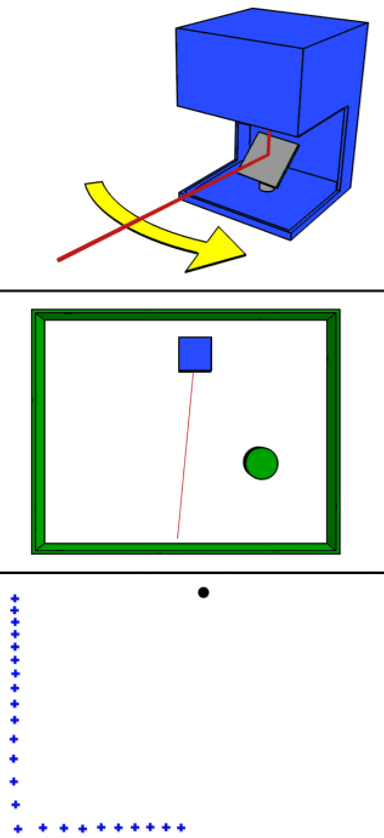
\includegraphics[width=4cm]{Lidar1}\label{fig:Lidar1}}}%
    \qquad
    \subfloat[]{{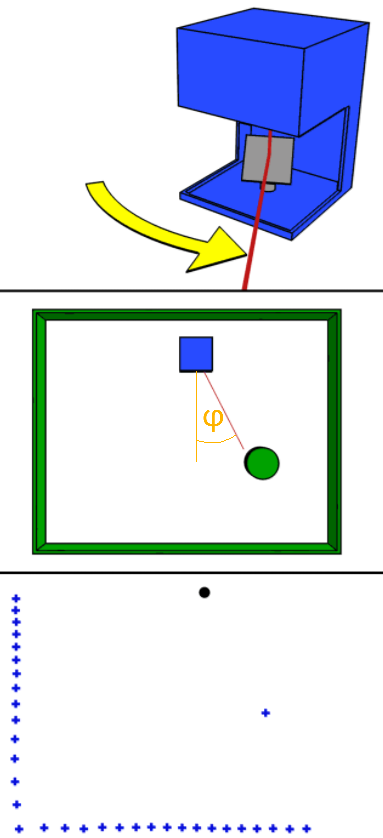
\includegraphics[width=4cm]{Lidar2Phi}\label{fig:Lidar2}}}%
    \qquad
    \subfloat[]{{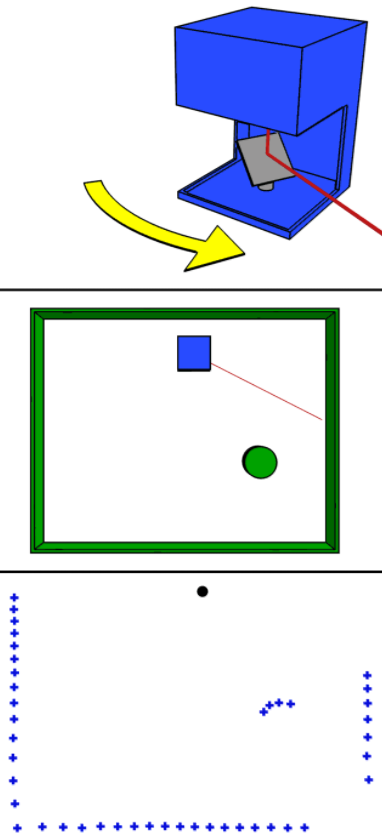
\includegraphics[width=4cm]{Lidar3}\label{fig:Lidar3}}}%
    \caption{Ablauf einer LiDAR-Messung von einem Sensor, der die Messimpulse im Uhrzeigersinn abgibt. Die Bilder stammen von \cite{bib:LidarPictures} und \ref {fig:Lidar2} wurde um den Winkel $\varphi$ erweitert.}\label{fig:Lidar}%
\end{figure}

Diese Methode liefert also eine gute horizontale Rundumsicht, welche aber innerhalb der vertikalen Sichtweite keinerlei Informationen bietet. Dies genügt in der Regel für simple Abstandserkennungen und Detektion von Hindernissen auf Höhe des Sensors. Möchte man jedoch Aussagen über das detektierte treffen oder braucht Informationen über andere vertikalen Ebenen, beispielsweise den Boden, muss man diese Methode noch erweitern. Dafür werden mehrere Lichtimpulse mit verschiedenen vertikalen Winkeln ausgesendet. Diese treffen die Umgebung dann mit unterschiedlicher Höhe womit die daraus resultierende Punktwolke eine dritte Dimension erhält. In Abbildung \ref{fig:LidarVertical} ist die seitliche Sicht auf einen LiDAR-Sensor mit mehreren vertikalen Lasern zu sehen.\\

\begin{figure}%
	\centering
    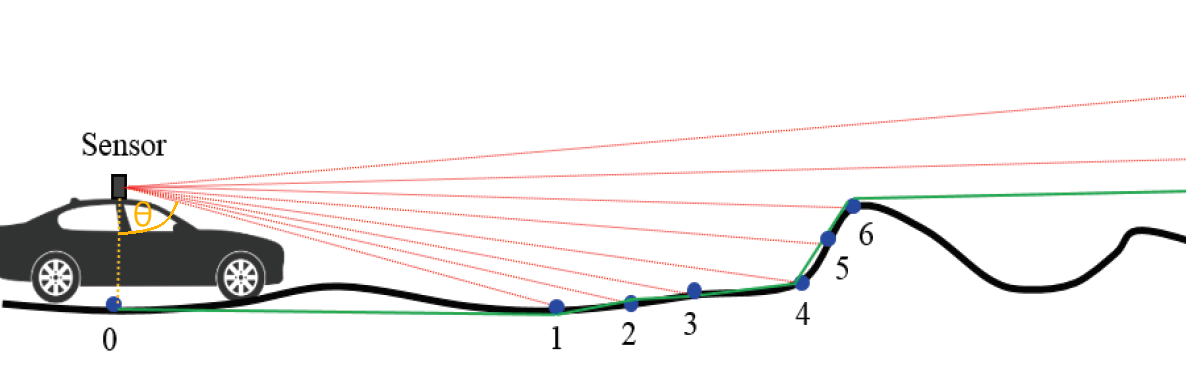
\includegraphics[width=14cm]{LidarVerticalTheta}
    \caption{Seitliche Sicht auf eine LiDAR-Messung mit mehreren, verital angeordneten Lasern. Die Abbildung stammt aus der Arbeit \cite{bib:FastGroundSeg} und wurde durch die Einzeichnung des Winkels $\theta$ erweitert.}
    \label{fig:LidarVertical}
\end{figure}

Wie schon erwähnt werden die erhaltenen Messdaten in eine Struktur konvertiert, die sich Punktwolke nennt. Dafür werden die Abstandsinformationen innerhalb eines bestimmten Koordinatensystems dargestellt. In der Regel wird dabei das \textit{Sphärische Koordinatensystem} verwendet. Darin wird jeder Punkt durch einen Abstand $r$ von einem Referenzpunkt und zwei dazugehörigen Winkel repräsentiert. Einer dieser Winkel ist dabei horizontal (Winkel $\varphi$) zu interpretieren und der andere vertikal (Winkel $\theta$). 

Nimmt man den Punkt \glqq 1\grqq{} aus der Abbildung \ref{fig:LidarVertical} als Beispiel, entspräche $\theta$ dem vertikalen Winkel. Dieser gibt den Winkel zwischen der gelben, gestrichelten Linie und der roten Linie an, die den Sensor und \glqq 1\grqq{} verbindet. Diese rote Linie repräsentiert den Abstand des Punktes vom Referenzpunkt, welcher der Position des Sensors entspricht. Der horizontale Winkel ist der Rotationswinkel des Sensors um seine eigene Achse (vgl. $\varphi$ in Abbildung \ref {fig:Lidar2}). Dieser wird vom Sensor bei jedem abgegebenen Impuls gemessen. Zusammenfassend kann also durch den vertikalen Winkel $\theta$ des Lichtimpulses, den horizontalen Winkel $\varphi$ des Sensors und dem gemessenen Abstand $r$ zum Sensor, der Punkt \glqq 1\grqq{} genau im Raum definiert werden.\\

Viele Anwendungen, die mit Punktwolken zu tun haben arbeiten jedoch mit dem kartesischen Koordinatensystem, so auch C.LABEL-VR. In diesem Koordinatensystem wird jeder dreidimensionale Punkt durch drei Koordinaten angegeben, nämlich der $x$-, $y$- und $z$-Koordinate. Ausgehend von den drei Werten des sphärischen Koordinatensystem können die drei kartesischen Koordinaten durch die Formeln in \ref{eq:SphToKart} berechnet werden. Auch hier steht $r$ für den Abstand zwischen dem Referenzpunkt und dem Punkt den man definieren will. $\theta$ steht für den vertikalen Winkel und $\varphi$ für den horizontalen Winkel, also den Rotationswinkel des Sensors um die eigene Achse.

\begin{subequations}
\begin{align}
        &x = r\sin\theta\cos\varphi \\
		&y = r\sin\theta\sin\varphi \\
		&z = r\sin\theta
\end{align}
\label{eq:SphToKart}
\end{subequations}

Durch die eben erklärte Definition der Messdaten in einem Koordinatensystem können diese Daten nun mit geeigneten Programmen (C.LABEL) als Punktwolke dargestellt werden. Darin ist dann jede einzelne Messung die der Sensor getätigt hat sichtbar. Somit kann der Mensch die Daten visuell analysieren und beispielsweise Zusammenhänge wie Objekte entdecken. Damit auch Computersysteme solche Objekte in diesen Daten erkennen können müssen sie erst lernen wie diese aussehen. Dazu muss eine Vielzahl an Punktwolken mit Hilfe eines LiDAR-Sensors aufgenommen werden und anschließend eine, vom Anwendungsfall abhängige, Anzahl an Punkten in dieser Wolke mit entsprechenden Klassifikationen versehen werden (Prinzip der Annotation aus Kapitel \ref{sec:Annotation}). Mit den annotierten Daten können nun Algorithmen, wie beispielsweise künstliche neuronale Netze (vgl. Kapitel \ref{sec:KNN}), lernen welche Zusammenhänge es in solchen Daten gibt und diese dann in nicht annotierten Daten wiedererkennen. Das Ziel von C.LABEL-VR ist es solche Daten in der virtuellen Realität zu visualisieren und Funktionen zur Verfügung zu stellen diese in der virtuelle Umgebung zu annotieren.




\chapter{C.LABEL VR}
\graphicspath{{Kapitel/Kapitel4_Hauptteil/Images/}}

Dieses Kapitel beschreibt die Virtual Reality Applikation \textit{C.LABEL-VR} und ist somit der Hauptteil dieser Arbeit. Das Ziel dieser Applikation ist es die Annotierung von Punktwolken, wie sie beispielsweise in C.LABEL möglich ist, innerhalb einer dreidimensionalen Umgebung zu realisieren. Dazu müssen zunächst Datenformate eingelesen werden, die Informationen über Punktwolken enthalten. Anschließend müssen aus diesen Daten Punktwolken erzeugt werden. Der Vorgang des Imports wird in Kapitel \ref{sec:ImportExport} näher beschrieben, die Erzeugung der Punktwolken in \ref{sec:Generierung}. Um sich in der virtuellen Umgebung durch diese Wolken bewegen zu können, wurden diverse Möglichkeiten zur Navigation entwickelt. Auf die Funktion dieser Möglichkeiten und deren Auswirkungen auf das Befinden des Menschen (\textit{Virtual Motion Sickness}) wird in Abschnitt \ref{sec:Navigation} eingegangen.\\

Anschließend geht es um die Annotierung der generierten Punktwolken. Annotierung bedeutet in diesem Kontext, dass die einzelnen Punkte der Wolken mit bestimmten Klassifikationen versehen werden, welche der Art des Objektes entsprechen, dem die Punkte zugehören. Ist der Punkt beispielsweise Bestandteil eines Autos, so wird er mit der Klasse \textit{Auto} versehen. Um diese Aufgabe erfüllen zu können wurden mehrere Arten der Annotierung entwickelt. Welche dies sind und wie sie realisiert wurden, wird in Abschnitt \ref{sec:Annotation} gezeigt. Das letzte Kapitel \ref{sec:UIMenu} beschäftigt sich mit der Benutzerschnittstelle der Applikation. Dieses wird auch \textit{User Interface} oder kurz \textit{\acrshort{acr:UI}} genannt. Dabei wird hauptsächlich auf die Funktionen des Menüs eingegangen welches man während des Labelns aufrufen kann. Ebenfalls wird erläutert welche Herausforderungen es bei der Erstellung von \acrshort{acr:UI}s in der virtuellen Realität gibt und wie diese bewältigt wurden. Zur Veranschaulichung aller Funktionen von C.LABEL-VR ist in der Abbildung \ref{fig:Workflow} der grobe \gls{glos:Workflow} in Form eines Diagramms abgebildet.

\begin{figure}%
	\centering
    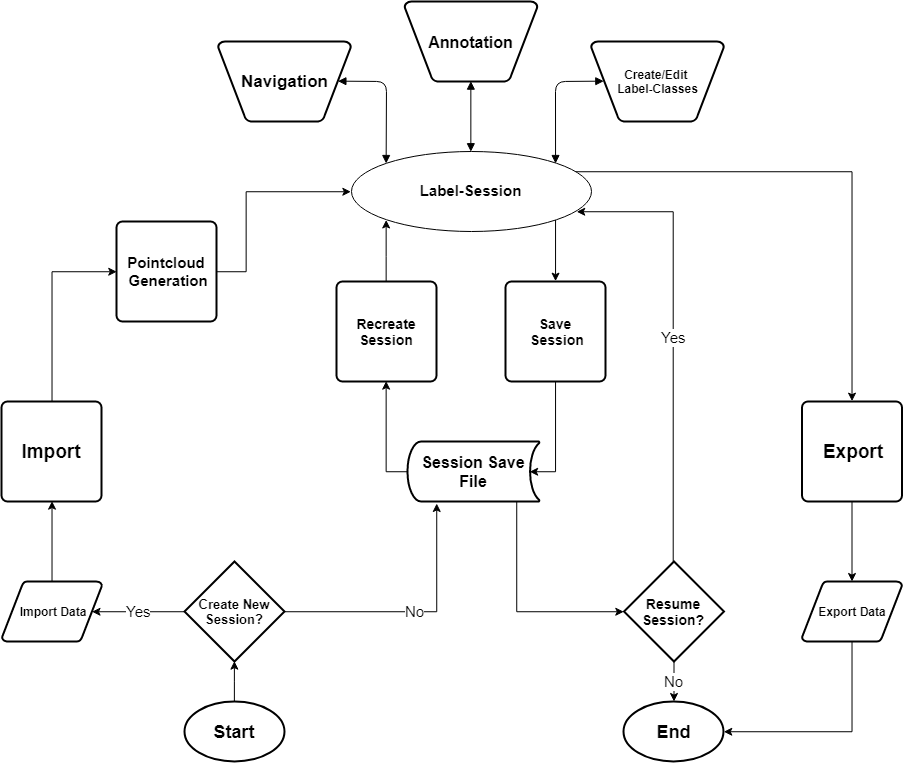
\includegraphics[width=13.5cm]{Workflow}
    \caption{\glslink{glos:Workflow} in C.LABEL-VR vom Import bis zum Export}
    \label{fig:Workflow}
\end{figure}


\section{Import und Export von Daten}
\label{sec:ImportExport}
Umfeldmodelle, welche in Form einer Punktwolke vorliegen, werden meist von einem Radar-, oder, wie in Kapitel \ref{sec:Lidar} gezeigt, von einem Lidar-Sensor aufgenommen. Die Informationen über diese Modelle, zum Beispiel die Positionen der einzelnen Punkte, werden in einem passenden Datenformat abgespeichert. Um welches Format es sich dabei handelt kann sehr unterschiedlich sein. In der Regel hängt es davon ab zu welchem Zweck die aufgenommenen Daten gebraucht werden und wie umfangreich diese Daten sind. Am häufigsten werden sie dafür verwendet um Lernalgorithmen und neuronale Netze (siehe Abschnitt \ref{sec:KNN}) zu trainieren. Automobilhersteller haben für solche Vorhaben natürlich unterschiedliche Konzepte und somit können auch die Formate der Daten unterschiedlich sein. Um die Applikation \textbf{C.LABEL-VR} für mehrere dieser Hersteller benutzbar zu machen, muss das Programm also mit verschiedenen Datenformaten umgehen können.\\ 

Innerhalb dieser Arbeit wurden mit zwei verschiedenen Arten von Daten gearbeitet. Das erste Format ist das PCD-Format (\textit{Point Cloud Data}). Die Bibliothek PCL(\textit{Point Cloud Library}) benutzt das Datenformat \textbf{PCD} um Informationen über Punktwolken zu verwalten. PCL ist eine sehr mächtige C++-Bibliothek, die in der Regel von jedem benutzt wird, der performante Algorithmen für Punktwolken entwickeln möchte. Auch C.LABEL generiert aus eingelesenen Daten PCD-Files um Funktionen der Point Cloud Library für die Wolken zu benutzen.\\

Das zweite Format ist das, von der HDF-Group bereitgestellte, HDF5-Format (\textit{Heterogeneous Data Format}). Es ist ausgelegt zum schnellen Erstellen und Auslesen von komplexen und großen Datenstrukturen. Welche Elemente diese Strukturen enthalten können wird später in Kapitel \ref{sec:HDF5} erklärt. Zur schnellen Bearbeitung großer Datenmengen ist dies ein gängiges Format und wird von den meisten Kunden von CMORE benutzt um Sensordaten zu verwalten. Deshalb wird es auch in C.LABEL-VR verwendet.\\

\subsection{Architektur}

Wichtig ist es also sowohl den Import, als auch den Export so modular wie möglich zu gestalten, dass C.LABEL-VR ohne große Änderungen  an der Hauptapplikation um neue Datenformate erweitert werden kann. Das Prinzip, das dafür entwickelt wurde, ist in Abbildung \ref{fig:ImportExport} dargestellt und wird im Folgenden näher erläutert. Die angesprochenen Erweiterungen um neue Datenformate werden als \textit{Addons} bezeichnet. Jedoch handelt es sich dabei nicht immer nur um eine Erweiterung eines, von Grund auf, neuen Datenformates. 
Bei Komplexen Datenformaten wie HDF5 kann der Entwickler die interne Struktur der Datei selbst bestimmen. Jede unterschiedliche Struktur muss auf unterschiedliche Weise eingelesen werden und braucht somit unterschiedliche Addons. Um die Erweiterbarkeit der Applikation sicherzustellen wurde der Import und der Export von der Hauptapplikation abgekapselt.

Dafür wurde eine interne Datenstruktur (kurz \acrshort{acr:IDS}) eingeführt, welche alle nötigen Informationen enthält, die für das \glslink{glos:Labeling}{Labeling} notwendig sind. Sie wird im späteren Kapitel \ref{sec:IDS} genauer vorgestellt. Der Vorteil dabei ist, dass die Hauptapplikation dadurch stets auf die gleiche Datenstruktur zurückgreifen kann. Sie bleibt somit unabhängig vom importierten Datenformat. Wird ein neues Import-Format eingeführt muss an der Hauptapplikation also nichts verändert werden. In der Abbildung \ref{fig:ImportExport} erkennt man, wie die Hauptapplikation (\textit{C.LABEL-VR Session}) nur mit internen Daten arbeitet und somit von den Import- und Exportdaten getrennt ist.\\ 

Jedes Import-Addon hat also zunächst die Aufgabe, seine jeweiligen Daten einzulesen und alle Informationen, die für die \acrshort{acr:IDS} notwendig sind, daraus zu extrahieren. Aus diesen Informationen können anschließend die entsprechenden Punktwolken generiert werden. Die Generierung wird in Kapitel \ref{sec:PclGenerate} erklärt. Beim Export ist es notwendig, dass die Struktur der Daten gleich bleibt, die vom Import-Addon eingelesenen wurden. Es sollen lediglich die \glslink{glos:Labeling}{Labeling}-Informationen aus der \acrshort{acr:IDS} hinzu- bzw. eingefügt werden. Aus der \acrshort{acr:IDS} kann das Export-Addon diese Informationen extrahieren und anschließend in die eingelesenen Daten exportieren. Die importierten Daten werden so allerdings überschrieben. Möchte man die Daten nicht überschreiben, müssen die Daten neu erstellt und mit den \glslink{glos:Labeling}{Labeling}-Informationen versehen werden. \\

Die Importierten Daten, beispielsweise HDF5, enthalten allerdings oft deutlich mehr Informationen, als für die interne Struktur notwendig. Diese Zusatzinformationen werden \textit{Metadaten} genannt. Für den Export bedeutet dies, dass man aus der internen Datenstruktur von C.LABEL-VR, die Struktur der anfangs eingelesenen Daten nicht wieder rekonstruieren kann, da die \textit{Metadaten} fehlen würden. Um dieses Problem zu lösen müssen die zusätzlichen Daten separat gespeichert werden. Dazu wurde eine erweiterbare Datenstruktur angelegt. In dieser kann man für jede Import-Struktur eine Metadatenstruktur anlegen. Das entsprechende Export-Addon kann die Metadaten dann verwenden um, zusammen mit den internen Daten, das gewünschte Exportformat zu rekonstruieren. \\

\begin{figure}%
	\centering
    \includegraphics[width=13.5cm]{Import_Export_Architecture}
    \caption{Das Import-Export-Prinzip in C.LABEL-VR}
    \label{fig:ImportExport}
\end{figure}

Zusammenfassend ist also folgendes zu tun, um die Benutzung ein neues Datenformates oder einer neuen Datenstruktur zu gewährleisten: Zunächst muss eine Importfunktion programmiert werden, die alle Informationen aus den gewünschten Daten ausliest. Anschließend muss diese Funktion das genormte, interne Datenformat (Kapitel \ref{sec:IDS}) erstellen und alle nötigen Informationen aus den eingelesenen Daten darin speichern.  Daraus können die entsprechenden Punktwolken dann generiert werden können. Falls es Daten gibt, die über diejenigen in der \acrshort{acr:IDS} hinausgehen, muss eine Metadatenstruktur angelegt werden, in welche die zusätzlichen Daten abgelegt werden können. Zuletzt ist eine Exportfunktion zu implementieren, welche die \glslink{glos:Labeling}{Labeling}-Informationen aus der internen Datenstruktur in die eingelesenen Daten exportieren kann. Außerdem muss sie in der Lage sein aus den internen- und den Metadaten das Ausgangsdatenformat wiederherzustellen, um die Daten als neue Files exportieren zu können. Im folgenden Kapitel soll dieses Prinzip konkret an einem HDF5-Beispiel gezeigt werden.

\subsection{HDF5-Beispiel}
\subsubsection{HDF5 Daten}
\label{sec:HDF5}
\subsubsection{Beispiel}

\section{Generierung einer Punktwolke}
\label{sec:Generierung}

\subsection{Interne Datenstruktur}
\label{sec:IDS}

\subsection{Generierung}
\label{sec:PclGenerate}
%session
%pointcloud
%...

%Koordinatensysteme

\subsection{Optimierung}
TODO
Methoden zur FPS-Steigerung

%-generell nichts teures in update mehthode
%	
%-gameobject find
%-getcomponent
%
%keine update oder start mehtode bei skripten der punkte
%collider trigger nicht bei den punkten sondern beim anderen object
%generell alle pollenden aktionen von den punkten entfernen
%
%
%(-clonen von prefabs statt neue instanzen von inbuilts)
%shared materials verwenden   kein material.color weil das eine kopie des materials erzeugt, welches dann einzeln gecallt werden muss
%
%gpu instancing bei den materials verwenden und forward rendering options

\section{Navigation}
\label{sec:Navigation}
\subsection{VR-Krankheit}
\subsection{Freier Flug}
\subsection{Teleport}

\section{Annotieren der Punktwolke}
\label{sec:Annotation}
\subsection{Einfache Pointer Annotation}
\label{sec:SimplePointerAnnotation}

\subsection{Cluster Annotation}
In einer Punktwolke mit mehreren tausend Punkten wird es für den Benutzer auf Dauer mühsam jeden Punkt einzeln zu Annotieren. Bei diesem Problem soll die \textit{Cluster Annotation} Abhilfe schaffen. Diese Art der Annotation soll selbstständig diejenigen Punkte in einen Cluster aufnehmen und sie mit der gleichen Klasse labeln, die zum gleichen Objekt gehören. Der Benutzer wählt hierfür, wie im vorherigen Kapitel \ref{sec:SimplePointerAnnotation} einen Punkt mit Hilfe des Pointers aus. Ausgehend davon werden umliegende Punkte untersucht, ob sie zum gleichen Objekt gehören wie der ausgewählte Startpunkt. Ist dies der Fall werden sie in den Cluster aufgenommen. Werden keine Punkte mehr aufgenommen bleibt der Endcluster übrig, welcher dann einem Objekt entspricht, zum Beispiel einem Auto. \\

Wissenschaftler beschäftigen sich intensiv mit solchen Verfahren zur Objektidentifizierung in dreidimensionalen Punktwolken. Ansätze, wie sie in \cite{bib:Segmentation1}, \cite{bib:Segmentation2} oder \cite{bib:Segmentation3} vorgestellt werden sind nur wenige von vielen. Die meisten haben aber ein ähnliches Vorgehen. Zuerst werden all diejenigen Punkte in der Wolke entfernt, die zum Boden gehören. So bleiben anschließend nur noch Punkte übrig, welche zu Objekten wie beispielsweise Autos, Häuser oder Straßenschilder gehören. Die übrigen Punkte können nun mit diversen Algorithmen zu Clustern zusammengefasst werden. Ein Beispiel für das Ergebnis eines solchen Verfahrens bietet die Abbildung \ref{fig:ClusteredCloud}. Im Folgenden wird vorgestellt wie die Cluster-Analyse in C.LABEL-VR funktioniert.

\begin{figure}%
	\centering
    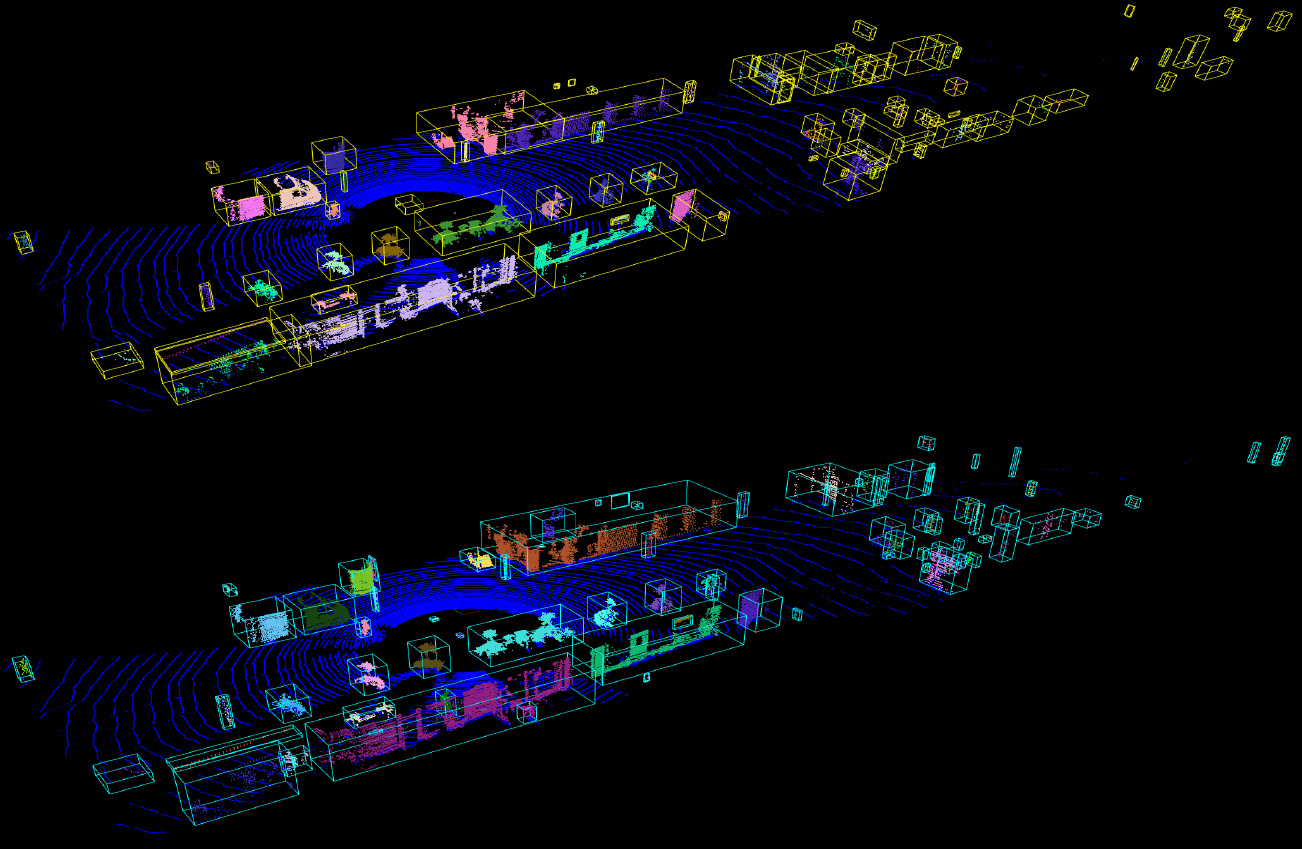
\includegraphics[width=15cm,height=7cm]{ClusteredPointCloud}
    \caption{Objektidentifizierung einer 3D-Punktwolke aus \cite{bib:Segmentation1}. Die Bodenpunkte der Wolke sind blau dargestellt und die Objekte sind mit Boxen gekennzeichnet.}
    \label{fig:ClusteredCloud}
\end{figure}

\subsubsection{Bodenpunkt-Analyse}
Wie schon erwähnt werden bei vielen Verfahren der Cluster-Analyse von Punktwolken zuerst die Bodenpunkte identifiziert. Dieses Verfahren wird auch in dieser Arbeit angewendet. Der Grund dafür ist, dass die Bodenpunkte nicht in das Suchverfahren nach Objektpunkten aufgenommen werden dürfen. Sie würden nicht nur die Suche nach echten Objektpunkten erschweren sondern auch das Ergebnis der Objektcluster verfälschen. Als Erklärung soll folgender, simpler Cluster-Algorithmus dienen:

\begin{enumerate}
\item Definiere einen Startpunkt $p$.
\item Ausgehend von $p$, suche alle Punkte innerhalb von Radius \(x\). 
\item Jeder gefundene Punkt ist ein neuer Startpunkt $p$.
\item Führe 2. aus bis es keine neuen Punkte $p$ mehr gibt.
\end{enumerate} 

Alle Objekte die auf dem Boden stehen, also deren Punkte nahe an Bodenpunkten sind, würden mit dem obigen Algorithmus die Bodenpunkte mit in den Cluster aufnehmen. Dies kann sogar dazu führen, dass 2 Objekte, die mittels Bodenpunkten miteinander verbunden sind zu einem Cluster zusammengefügt werden. Darum müssen die Bodenpunkte von den Objektpunkten getrennt werden um eine exakte Objekterkennung zu garantieren.

Die Segmentierung des Bodens wird in C.LABEL-VR nach dem Einlesen des internen Datenformates ausgeführt, also zwischen Import Addons und PCL Generator (siehe Abbildung \ref{fig:ImportExport}). Beim Erstellen der Punktwolken ist also schon bekannt welcher Punkt ein Bodenpunkt ist und welcher nicht. Dazu wird im internen Datenformat das Attribut für die Bodenpunktkennzeichnung mit dem entsprechenden Wert versehen (vgl. Abschnitt \ref{sec:IDS}). Wie diese Werte ermittelt werden ist im Folgenden erklärt.\\

Als Basis für die Bodenpunktanalyse in C.LABEL-VR wurde das \textit{Ground Plane Fitting}-Verfahren (GPF) aus \cite{bib:Segmentation1} verwendet. Ist im weiteren Verlauf dieser Arbeit die Rede von GPF, ist immer der Ansatz der eben zitierten Arbeit gemeint. Ziel dieses Verfahrens ist es ein mathematisches Modell einer Ebene zu errechnen, welches den Boden repräsentieren soll. Anschließend kann von jedem Punkt der Abstand zu dieser Ebene ermittelt werden. Ist der Abstand eines Punktes kleiner als ein definierter Wert, so handelt es sich bei ihm um einen Bodenpunkt.

Die Punktwolke, die analysiert werden soll, wird dabei zunächst in eine Anzahl an $N_{segs}$ Segmenten aufgeteilt. Der Algorithmus zur Identifizierung der Bodenpunkte wird für jedes dieser Segmente ausgeführt. Der Grund für diese Segmentierung ist die mögliche Unebenheit der Bodenfläche. Soll eine wellige Oberfläche von einer Ebene repräsentiert werden kommt es zu ungenauen Ergebnissen. Wird aber für jedes Segment der Punktwolke eine eigene Ebene ermittelt so verbessert sich das Ergebnis der Bodenpunktanalyse, wie in Abbildung \ref{fig:Segments} zu sehen ist.

\begin{figure}%
	\centering
    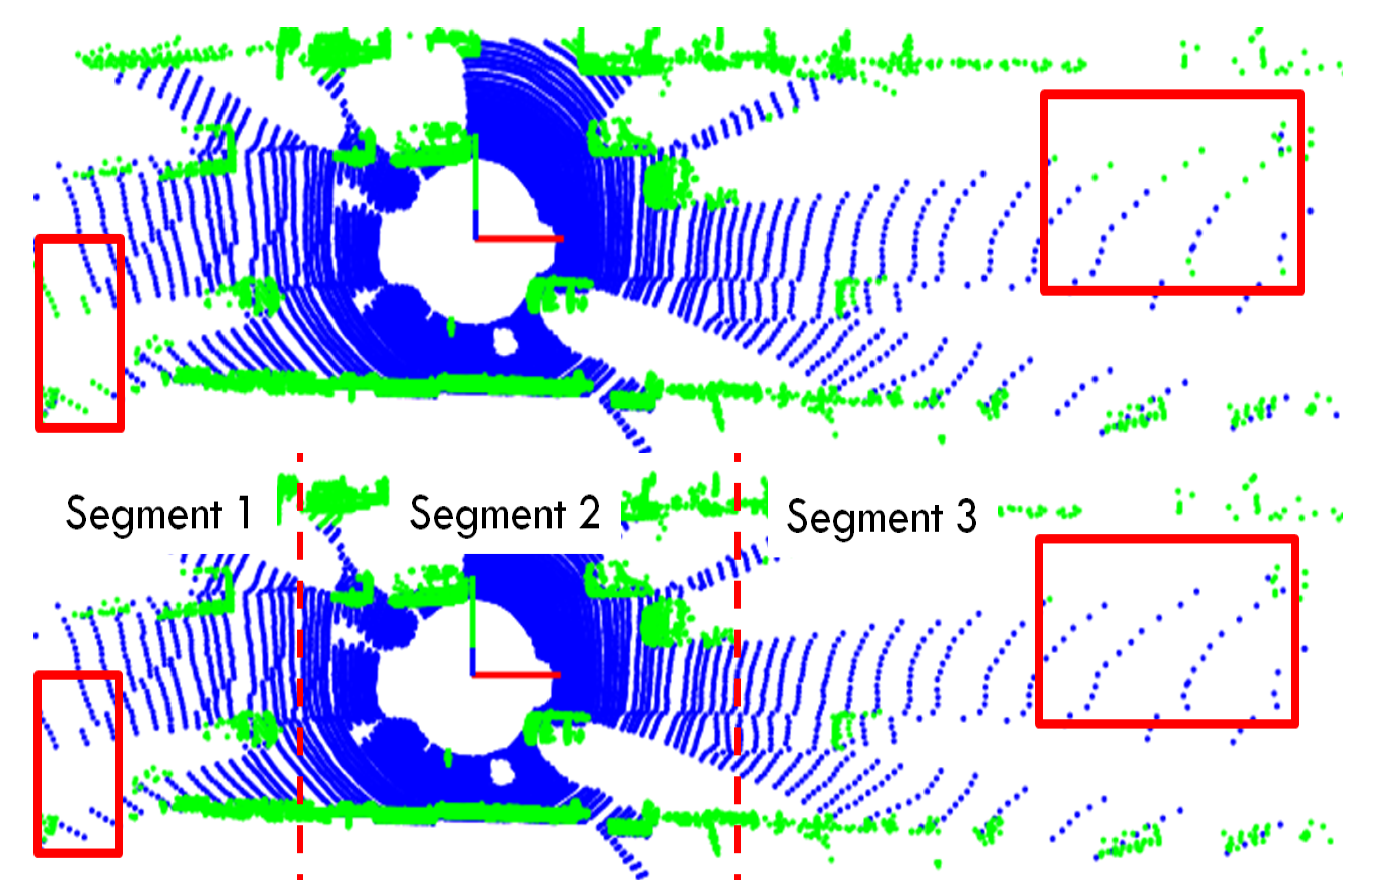
\includegraphics[width=14cm,height=6cm]{Segments}
    \caption{In \cite{bib:Segmentation1} wird gezeigt, dass die Segmentierung einer Punktwolke zu einem besseren Ergebnis der Bodenpunktanalyse führt. Die obere Abbildung ist dabei ohne Segmentierung und die untere mit Segmentierung. Bodenpunkte sind blau und Objektpunkte in grün dargestellt. Die roten Rechtecke kennzeichnen den Bereich in dem die Analyse schlechter bzw. besser ist.}
    \label{fig:Segments}
\end{figure}

Beim GPF-Verfahren wurden Punktwolken in 3 große Segmente entlang der $x$-Achse eingeteilt, da diese Achse der Fahrtrichtung des Autos entspricht. Damit wurden für die Testdaten, die CMORE für diese Arbeit zur Verfügung stellte, keine zufriedenstellenden Ergebnisse erzielt (vgl. Abbildung \ref{fig:WrongSegments}). Das Problem ist, dass sich durch eine zu simple Segmentierung entweder zu viele oder zu wenige Bodenpunkte in einem Sektor befinden können. Bei zu vielen Bodenpunkten kann es sein, dass der Boden nicht linear verläuft. Auf der linken Seite des Autos könnte sich beispielsweise eine Anhöhe befinden und auf der rechten Seite ein flaches Gelände. In diese Unebenheit kann keine richtige Ebene eingesetzt werden. Bei zu wenigen Bodenpunkten kann es sein, dass der Algorithmus die Ebene an Objekte annähert. Handelt es sich bei solchen Objekten beispielsweise um eine senkrechte Wand, können die vielen hohen Punkte die Ebene senkrecht werden lassen(siehe Abbildung \ref{fig:WrongFit}).\\

\begin{figure}%
    \centering
    \subfloat[Segmentierung anhand potentieller Bodenpunkten]{{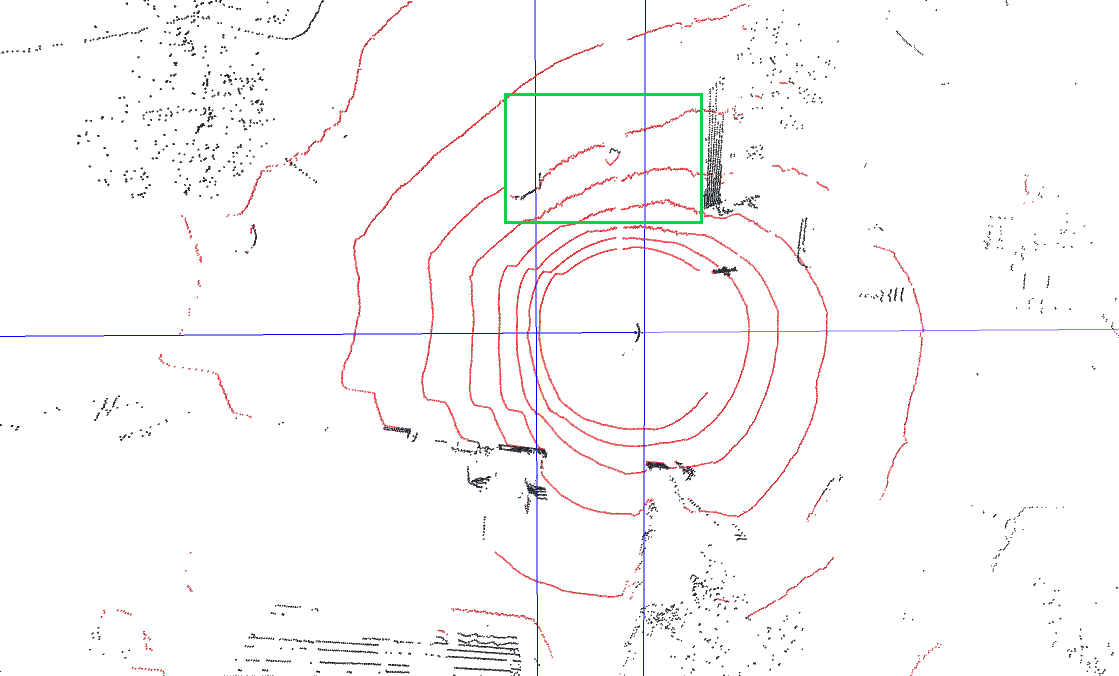
\includegraphics[width=7cm]{GroundSeg_BirdeyeWithSectors2}\label{fig:RightSegments}}}%
    \qquad
    \subfloat[Segmentierung anhand Koordinaten entlang der $x$-Achse]{{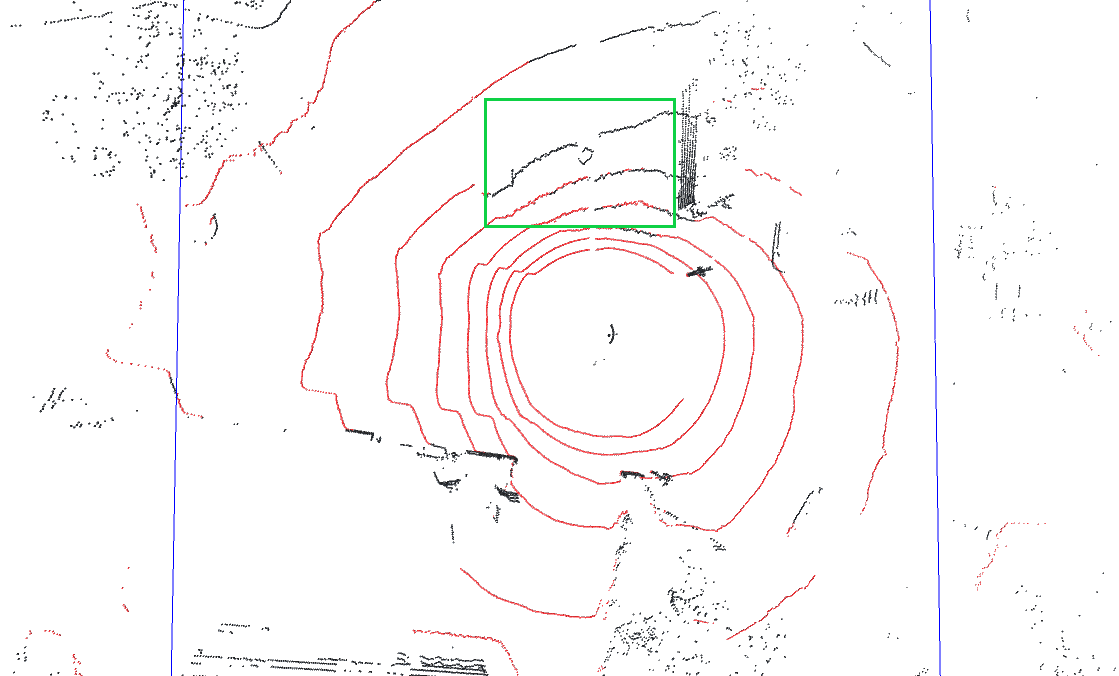
\includegraphics[width=7cm]{GroundSeg_BirdeyeWithWrongSectors2}\label{fig:WrongSegments}}}%
    \caption{Vergleich der Segmentierungsmethoden zur Bodenpunktanalyse aus \cite{bib:Segmentation1} und C.LABEL-VR. Bodenpunkte sind rot, alle anderen schwarz. Die blauen Linien stellen die Trennung der Segmente dar. Die grünen Boxen markieren den Bereich, in dem man den Unterschied der beiden Methoden bei der Bodenpunkterkennung sieht.}\label{fig:Segmentation}%
\end{figure}

\begin{figure}%
	\centering
    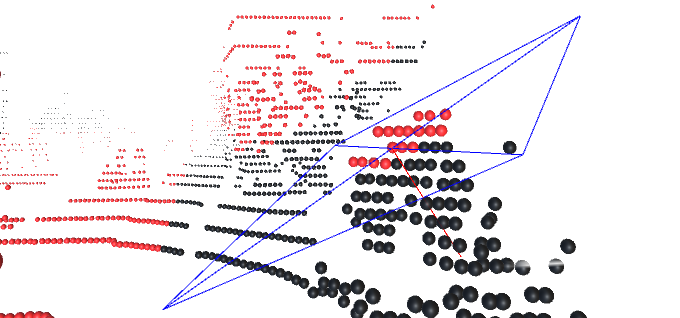
\includegraphics[width=15cm,height=5cm]{WrongFit}
    \caption{Bei zu wenigen Bodenpunkten in einem Segment passt sich die Ebene den falschen Punkten an.}
    \label{fig:WrongFit}
\end{figure}

Darum wurde in dieser Arbeit ein Verfahren entwickelt, dass die Segmente nicht anhand ihrer Größe einteilt sondern nach der Anzahl der potentiellen Bodenpunkte, welche die Segmente enthalten (siehe Algorithmus \ref{alg:Segmentation}). Potentielle Bodenpunkte sind diejenigen Punkte, welche sich in einem bestimmten Höhenbereich befinden. Der Höhenbereich wurde auf -0.5m bis 0.5m festgelegt. Das bedeutet alle Punkte, deren Höhenwert sich innerhalb des Wertebereichs befindet, sind potentielle Bodenpunkte. Das Segmentierungsverfahren erstellt nun die Segmente so, dass sich in jedem Segment gleich viele dieser potentiellen Bodenpunkte befinden. 

Dazu werden alle Punkte des gesamten Segments nach ihrem $x$-Wert sortiert und anschließend wird durch diese Menge an sortierten Punkten iteriert. Bei jeder Iteration wird geprüft ob der aktuell betrachtete Punkt ein potentieller Bodenpunkt ist oder nicht. Ist das der Fall wird eine Zählvariable erhöht. Übersteigt der Wert dieser Variable die Anzahl an potentiellen Bodenpunkten, die in einem Segment sein sollen, werden zukünftig betrachtete Punkte in ein neues Segment aufgenommen. Die Zählvariable wird anschließend wieder auf Null gesetzt um im neuen Segment die potentiellen Bodenpunkte erneut zu zählen.    

\begin{algorithm}
  \caption{Algorithmus zur Einteilung einer Punktwolke in $N_{segs}$ Segmente}
\label{alg:Segmentation}
  \begin{algorithmic}[1]
    \Inputs{\textbf{$\textbf{P}$} : Menge aller Punkte\\
    				$N_{segs}$ : Anzahl der Segmente}
    \Initialize{$\textbf{S}$ : Menge aller Segmente mit ihren Punkten\\
    			$\textbf{P}_{pot}$ : Menge aller potentiellen Bodenpunkte\\
    			$C_{segs} :$ Zähler des aktuellen Segments\\
    			$C_{points} :$ Zähler der Bodenpunkte des aktuellen Segments\\
    			$N_{gpps} :$ Anzahl der potentiellen Bodenpunkte pro Segment\\}

   	\State \textbf{MainLoop:}
   	\State $\textbf{P}_{sorted} = \Call{\textbf{SortAscendingOnXValue}}{\textbf{P}}$;
  	\State $\textbf{P}_{pot} = \Call{\textbf{GetPointsBetweenHeightValues}}{-0.5, 0.5, \textbf{P}_{sorted}} $;
  	\State $N_{gpps} = \ceil*{\frac{|\textbf{P}_{pot}|}{N_{segs}}}$; 
  	\State $C_{segs} = C_{points} = 0$;
    \For{$i=1 : |\textbf{P}_{sorted}| $}
      	\If{$p_i.yValue \geq 0$}
      		\State $\textbf{S}[C_{segs}] \gets p_i$;
      	\Else
      		\State $\textbf{S}[C_{segs}+1] \gets p_i$;
      	\EndIf

      	\If{$p_i \in \textbf{P}_{pot}$}
      		\State $C_{points}++$;
      	\EndIf
      	
		\If{$C_{points} \geq N_{pps}$}
      		\State $C_{points} = 0$;
      		\State $C_{segs} += 2$;
      	\EndIf      	
    \EndFor

  \end{algorithmic}
\end{algorithm}

Zusätzlich zu der Segmentierung aus \cite{bib:Segmentation1} wurden die Segmente noch durch die $y$-Achse geteilt, um den vorher angesprochenen Problemfall der unterschiedlichen Geländebeschaffenheiten links bzw. rechts vom Auto auszugleichen. Dazu wird bei jeder Iteration der $y$-Wert des betrachteten Punktes geprüft. Punkte mit einem größeren Wert als Null werden in ein anderes Segment aufgenommen als solche mit kleinerem Wert. Das Ergebnis und der direkte Vergleich mit der normalen GPF-Methode ist in Abbildung \ref{fig:RightSegments} zu sehen.\\

Nach dem die Segmentierung der Punktwolke vorgenommen wurde, muss nun die Bodenebene für jedes Segment berechnet werden. Die Definition dieses Vorgehens ist in Algorithmus \ref{alg:GroundPoints} gegeben. Auch dafür wurde die GPF-Methode aus \cite{bib:Segmentation1} als Basis hergenommen. Zuerst werden gewisse Startpunkte ermittelt, welche auch \textit{Seedpoints} bzw. \textit{Seed-Punkte} genannt werden. Laut GPF werden diese Punkte durch den \textit{LPR}-Wert (\textit{lowest point representative}) ermittelt. Um diesen Wert zu berechnen wird zunächst eine Anzahl an  $N_{LPR}$ Punkten definiert. Danach werden die $N_{LPR}$ tiefsten Punkte des Segments genommen und der Durchschnitt der Höhenwerte dieser Punkte berechnet. Alle Punkte des Sektors die eine maximale Höhendifferenz $T_{init}$ zu diesem Wert haben sind Seed-Punkte. 

Dieses Vorgehen ist allerdings anfällig für Rauschen in Form von sehr tiefen Punkten. Befinden sich im Segment also fälschlicherweise Punkte, die tief unter dem Boden sind, verfälschen diese die richtige Berechnung des Durchschnittshöhenwerts. Deshalb wurden in C.LABEL-VR für die Berechnung Durchschnittshöhenwerts LPR nicht die $N_{LPR}$ tiefsten Punkte hergenommen, sondern alle potentiellen Bodenpunkte die sich in dem Segment befinden. Aus diesem Durchschnittshöhenwert und der maximal zulässigen Differenz $T_{init}$ werden, wie schon beschrieben, die Startpunkte ermittelt. Die Formale Beschreibung dieses Vorgehens ist ebenfalls in Algorithmus \ref{alg:GroundPoints} zu sehen (GetInitialSeedPoints).\\

Mit diesen Startpunkten kann nun die erste von $N_{iter}$ Schätzungen für die Bodenebene berechnet werden. Eine Ebene $E$ kann definiert werden durch einen Vektor $\vec{n}$ der Senkrecht auf der Ebene steht (Normalenvektor) und einem Punkt $p$ der auf der Ebene liegt. Ziel ist es nun diese beiden Komponenten so zu berechnen, dass die dadurch definierte Ebene bestmöglich in Seed-Punkte passt. Für den Punkt $p$ kann man den einfach Durchschnitt $\hat{s}$ aus allen Elementen der Menge aller Seed-Punkte $S$ nehmen. Dieser Punkt repräsentiert den Ursprung der Ebene und bietet sich deshalb an weil man ihn bei späteren Berechnungen wiederverwenden kann (siehe Gleichung \ref{eq:Covar}).

Die Berechnung des Normalenvektors $\vec{n}$ ist dagegen deutlich aufwändiger. Zunächst wird die Streuung aller Punkte $s \in S$ untersucht. Dazu wird eine Kovarianzmatrix $C$ des Ranges $R^{3x3}$ berechnet, welche die Streuung der Seedpoints repräsentiert. Diese Matrix kann nun auf geometrische Eigenschaften untersucht werden, beispielsweise welcher Vektor die kleinste Streuung repräsentiert und somit als $\vec{n}$ verwendet werden kann.

\begin{equation} 
C=\sum_{i=1:\vert S\vert }(s_{i}-\hat{s})(s_{i}-\hat{s})^{T}
\label{eq:Covar} 
\end{equation}

Im Allgemeinen gilt für eine Matrix Folgendes: \glqq \textit{Eine Matrix definiert durch $y=A*x$ eine lineare Abbildung $R^m \to R^n$. Der Hauptberuf einer Matrix ist, aus einem Vektor einen anderen zu machen. Im Allgemeinen ändert die Matrix dadurch Richtung, Betrag (und sogar
Dimension) eines Vektors. Matrixzerlegungen spalten die Aktion der Matrix in leichter zu durchblickende Einzelschritte auf}\grqq \cite{bib:Decomposion}. Aus diesen Einzelschritten können geometrische Informationen extrahiert werden. Bei der GPF-Methode wird $C$ durch die Singulärwertzerlegung gespalten. Dieses Verfahren wird auch \textit{Singular Value Decomposion} (SVD) genannt. Wie in \cite{bib:SVD} gezeigt, wird bei SVD eine Matrix $A \in R^{mxn}$ in 2 orthogonale Matrizen $U \in R^{mxm}$ und $V\in R^{nxn}$ und eine diagonal Matrix $\Sigma$ zerlegt, sodass die Gleichung \ref{eq:SVD} erfüllt wird. Der Normalenvektor $\vec{n}$ der gesuchten Ebene ist gegeben durch die dritte Spalte der Matrix $U$ \cite{bib:SVDforFitting}.

\begin{equation} 
A=U \Sigma V^T
\label{eq:SVD}
\end{equation}

%Die Singulärwertzerlegung kann, wie schon angesprochen, für beliebige Matrizen in $R^{nxm}$ verwendet werden. Da die berechnete Kovarianzmatrix $C$ aus der Gleichung \ref{eq:Covar} immer eine $3x3$ Matrix ist, kann die Matrix aber auch in ihre Eigenwerte und Eigenvektoren zerlegt werden. Der kleinste Eigenwert dieser Zerlegung entspricht dem gesuchten Normalenvektor $\vec{n}$. Wie man in \cite{bib:SVD} sehen kann, ist ein Schritt zur Singulärwertzerlegung die Berechnung der Eigenwerte einer Matrix. Die reine Berechnung der Eigenwerte erfordert also weniger Rechenschritte als die Singulärwertzerlegung und bietet bei der Analyse vieler Punktwolken eine kürzere Dauer der Berechnungen. Auch Quellcode-Bibliotheken wie \textit{Geometric Tools Engine} benutzten dieses Verfahren um eine Ebenenmodell in einer Menge von Punkten zu berechnen \cite{bib:g3sharp}. Deshalb wurde es auch in C.LABEL verwendet.\\

Die gesuchte Ebene ist nun durch den Punkt $p$ und den Vektor $\vec{n}$ nun eindeutig definiert. Nun kann der Abstand jedes Punktes des Segments zu seiner orthogonalen Projektion auf der definierten Ebene berechnet werden. Dieser Abstand wird dann mit einem Schwellwert $T_{plane}$ verglichen, welcher zu Beginn der Berechnung definiert werden muss. Ist der Abstand eines Punktes kleiner als der Schwellwert so handelt es sich bei ihm um einen Bodenpunkt. In C.LABEL-VR wird solch ein Punkt vorläufig als Bodenpunkt markiert und in die Menge an neuen Seed-Punkten aufgenommen. Mit diesen neuen Seed-Punkten wird anschließend die nächste von $N_{iter}$ Berechnungen der Bodenebene getätigt(vgl. Algorithmus \ref{alg:GroundPoints}).

\begin{algorithm}
  \caption{Algorithmus zur Identifizierung von Bodenpunkten eines Punktwolken-Segments}
\label{alg:GroundPoints}
  \begin{algorithmic}[1]
    \Inputs{\textbf{$\textbf{P}$} : Menge aller Punkte der Wolke\\}
    \Initialize{\textbf{$\textbf{P}_{seeds}$} : Menge aller Seed-Punkte\\
    			%$N_{segs} :$ Anzahl der Segmente\\
    			$N_{iter} :$ Anzahl der Iterationen\\
    			$T_{init} :$ Distanzgrenzwert der initialen Seed-Punkte\\
    			$T_{plane} :$ Distanzgrenzwert zur geschätzten Ebene}
   	\State \textbf{MainLoop:}
  	\State $\textbf{P}_{seeds}$ = \Call{\textbf{GetInitialSeedPoints}}{$\textbf{P}$, $T_{init}$};
    \For{$i=1 : N_{iter}$}
      \State $plane$ = \Call{\textbf{FitPlaneIntoPoints}}{$\textbf{P}_{seeds}$};
      \State \Call{Clear}{$\textbf{P}_{seeds}$};
      \For{$j=1 : |\textbf{P}|$}
      	\State $distance$ = \Call{\textbf{GetDistanceToPlane}}{$plane$, $p_k$};
      	\If{$distance < T_{plane}$}
      		\State $p_k.groundpoint = true$;
      		\State $\textbf{P}_{seeds} \gets p_k$
      	\Else
      		\State $p_k.groundpoint = false$;
      	\EndIf
      \EndFor
    \EndFor
    \\
    \State \textbf{GetInitialSeedPoints:}
    \Initialize{\textbf{$\textbf{P}_{low}$} : Alle tiefen Punkte aus $\textbf{P}$\\
   			$H_{avg}$ : Durchschnittshöhe alle Punkte aus $\textbf{P}_{low}$}
    \For{$i=1 : |\textbf{P}|$}
    	\If{$p_i.height < 0.5 \And p_i.height > -0.5$}
    		\State $\textbf{P}_{low} \gets p_i$
    	\EndIf 
    \EndFor
    \State $H_{avg} = \Call{\textbf{GetAverageHeight}}{\textbf{P}_{low}}$;
    \For{$i=1 : |\textbf{P}|$}
    	\If{$p_i.height < T_{init}$}
    		\State $\textbf{P}_{seeds} \gets p:i$;
    	\EndIf 
    \EndFor
  \end{algorithmic}
\end{algorithm}

\subsubsection{Cluster-Analyse}


\section{User Interface}
\label{sec:UIMenu}
\subsection{Ingame Menu}
%\subsection{Movement}
%\subsection{Labelclasses}




\chapter{Schluss}

\section{Zusammenfassung}

\section{Herausforderungen}

\section{Ausblick}



%\chapter{Ab hier kommen Inhalte für CopyPaste}
%\chapter{Sections and Paragraphs}

\section{Section}
Inhalt des ersten Abschnitts
\subsection{Subsection}
\label{lab1}
Inhalt des ersten Unterabschnitts
\paragraph{Paragraph!?}
\subparagraph{Unterparagraph!?}

\section{Referenz}
Wie in \ref{lab1} geschrieben.

\chapter{Lists}

\begin{enumerate}
\item erstens
\item zweitens
\begin{itemize}
\item unter erstens
\item unter zweitens
\item[+] Pro
\item[-] Contra
\end{itemize}
\item drittens\\
Das Zeichen \verb|\\| \\ forciert eine neue Zeile.
\end{enumerate}


\chapter{Tabellen}
\begin{tabular}{|l|l|}
left alligned & left alligned----------\\
left alligned------- & left alligned\\
\end{tabular}

\begin{tabular}{|r|r|}
------right alligned & right alligned\\
right alligned & --------right alligned\\
\end{tabular}

\begin{tabular}{|c|c|}
center alligned & center alligned\\
center alligned & center alligned\\
\end{tabular}

\begin{tabular}{|l|r|c|}
left alligned & right alligned & center alligned\\
\end{tabular}

\chapter{Figures}

\begin{figure}[h] %h=here	t=top	b=bottom	p=seperate page 
\centering	%if not centered then left aligned

\includegraphics[width=1\textwidth]{Main_Images/cmoreLogo}
\caption{Here is my image}
\label{image-myimage}
\end{figure}

\chapter{Equations}

$1+2=3$ \\
$$1+2=3$$
\begin{equation}
1+2=3
\end{equation}
\\
\begin{eqnarray}
x_1^2 & = & 1+2+3 \\
& = & \sqrt{6}
\end{eqnarray}


\chapter{References}
This is a reference.\cite{Testzitat}

This is a website reference.\cite{TestWebsite}
%\chapter{Ab hier enden Inhalte für CopyPaste}


\appendix
\chapter{Appendix Title}
%\input{chapters/appendix}



\bibliographystyle{IEEEtran}
\bibliography{Masterarbeit}

\end{document}